\documentclass[12pt,a4paper]{thesis}
\usepackage[a4paper,left=1.4in,right=.75in,top=1in,bottom=.75in, includehead]{geometry}
\usepackage[latin1]{inputenc}
\usepackage{amsmath}
\usepackage{amsfonts}
\usepackage{amssymb}
\usepackage{graphicx}
\usepackage[doublespacing]{setspace}
\usepackage[authoryear]{natbib}
\usepackage{url}
\usepackage{rotating}
\usepackage{float}
\usepackage[toc,page]{appendix}
\begin{document}

\title{Spatial Interaction Simulation Methods for Ancient Settlement Distributions in Central Italy}

\maketitle

\tableofcontents

\listoffigures

\listoftables

\chapter{Introduction}
\section{General Overview}

\paragraph{}
Human Landscapes are created by the necessary struggle of people to meet their social and economic needs.  Eckbo states, ``Historically, these objectives have run a gamut from utility through increasing convenience, comfort, and luxury to the more conscious and ostentatious display of wealth and power'' \citeyearpar[p. 8]{Eckbo69}. Thus, as societies have settled and developed urban communities, human culture intensified, which in turn magnified the relationship between the people and the earth. The result is that the landscape is created by human decisions whether or not it was their intent to do so \citetext{\citealp[3-8]{Eckbo69}; \citealp[161]{AnsWilSch01}}. These decisions result in connections between people, places, and groups, producing a network of spatial interactions. More specifically, network science, which is the study of links and nodes on a graph and the attributes that arise from their interconnectedness, provides methods for visualizing and investigating settlement structures throughout the landscape. Networks allow for an environment in which many individual actors or settlements interact with each other simultaneously, creating a summation of those influences at each node. They also have the ability to represent various levels of structure \cite[9-10]{KnoKuk92}. Together these characteristics provide the ability to take static components and weave them together to more closely look at how a system that was truly dynamic in nature would have evolved.

\paragraph{}
Space is, and has always been, a pervasive  element in the daily routine of humans which can be studied through a range of forms, from symbolic manifestations to more physical representations \cite[p. 282]{Harvey06}. Naturally any study focused on the development of humanity is geographic by nature since, as a species, we have proliferated at all scales. These two points extend  to research on the distribution of excavated remains, features amongst remains, and the examination of spatial interaction between them. As a result, it is sensible to apply a geographer's toolbox to certain questions within the archaeology domain \cite[p. 39-42]{Kantner08}

\paragraph{}
Yu-Fi Tuan \citeyear{Tuan76}, writes, ``If history is a pillar of the humanities then historical geography ought to be the pillar of humanistic geography''(272). Following this line of thinking, archaeology and humanistic geography can be thought of as overlapping, and thus sharing a common goal of building a history of humans. Tuan also writes, ``The vivid depiction of a region is perhaps humanistic geography's highest achievement'' (273). As such, it can be argued that through spatial analysis we will enrich our perception of a region and therefore help answer broader questions about how a place becomes defined through the larger landscape within which it exists (274).

\paragraph{} 
The purpose of this research is to explore the spatial distribution of early Etruscan states within a geographic network structure in order to shed light on how space conditioned their development  and then subsequently influenced how these sites interacted with each other. Specifically, this research will focus on how these spatial effects  pertain to the site known as Poggio Civitate (Murlo), which is located approximately 25km southeast of Siena, Italy. By considering the entire region of ancient Etruria, which coincides heavily with the modern Italian province of Tuscany, it will be possible to examine Poggio Civitate's individual characteristics as well as its relationship to other settlements within a cohesive Etruscan society. It is hoped that new evidence will be contributed towards existing theories which seek to explain the nature of this wealthy settlement which was abruptly destroyed and has henceforth remained uninhabited.

\paragraph{}
Quantitative modeling will be embraced as the analytical framework within which to carry out the proposed spatial 
analysis. Large multi-dimensional datasets quickly become complicated and conceptually difficult to manage. Models become a necessity to mitigate these complexities. They also act as a tool to develop hypotheses since the models can be parameterized in such a way to test existing and new theories. By employing a common language they increase dissemination and communication within and between fields \citep{Wyl09}. Quantitative modeling's merits within archaeology are summarized below by \citep{ERK12}:

\begin{singlespace}
\begin{quote}
        ``Despite our best attempts at deducing relationships from the artefacts found at them [sites], there is often little direct information about how sites interact. Quantitative modelling provides one response to this challenge. Good quantitative modelling can be insensitive to poor data, make assumptions and biases clear and debatable, and can allow us to provide possible answers to questions that could not be asked any other way. In the best case, such answers can be checked later from the archaeological record.''(1)
\end{quote}
\end{singlespace}

\paragraph{}
Three conceptually unique techniques will be employed in order to simulate relative spatial interactions amongst the sites in the study area: an agent-based model, a radiation analogy model, and a Hamiltonian gravitational model. As a consequence, each model provides varying interpretations of spatial interaction by approaching the problem from 3 different perspectives. A multitude of models offers the ability to compare and contrast different nuances of a phenomenon using the same spatial inputs. Furthermore, different representations that yield varying yet similar results will provide assurance that we are indeed capturing the intended actions.
Subsequent chapters will elaborate on the concepts presented here. Chapter two will begin with a brief history of the Etruscans  and how Poggio Civitate fits into that narrative. It will then introduce the concept of spatial interaction theory and spatial interaction modeling, followed by a review of spatial interaction studies within the field of archaeology. A final product of Chapter two will be the selection of the three models that will be employed in this research.  Next, Chapter three will provide an explicit statement of the research goals and hypotheses that pertain to this research. Chapter four can be broken into three sections; the first will establish the input data that will be used for all three models while the second will provide in-depth description of how each model will be used to simulate networks, and, finally, the third section will establish the appropriate metrics to analyze the networks . The resulting networks and their properties will be reported in Chapter 5. Finally, the discussions and conclusions (Chapters Six and Seven) will provide a holistic summary of the research overall, a comparison of the three models, the implications each has regarding specific research questions, and suggestions for future research.

\chapter{Literature Review}
\section{History of the Etruscans and Poggio Civitate}

\paragraph{}
Etruria generally refers to the society that dwelt in ancient Italy from the pre-historic era through to the flourishing of the Roman civilization. Indeed there is much evidence that Etruscan culture was adopted by the Romans and that  these two cultures co-existed before the expansion of the Romans and subsequent decline of the Etruscans \cite[30-32, 56-60]{Scu80}. The height of Etruscan culture included complex cities, naval prowess, and intricate craftsmanship. Evidence for occupation within Etruria exists as early as about 4-5 millenniums BCE though it is not until much later that  distinct Etruscan culture emerged. Four general time periods can be assigned in the assessment of Etruscan historical development: the Late Bronze Age (c. 1300-900 BCE), the Villanovan period (c. 900-750 BCE), the Orientalizing period (c. 750-580 BCE), and the Archaic/Classical period (c. 580-400 BCE). The geographic extent covered by the Etruscans (Figure \ref{fig:etruria}) is usually prescribed as Central Italy, though in reality their territory covered a wider area which encompassed modern Lazio, Tuscany, and parts of Umbria, Campania, Emilia and Veneto \cite[21, 38]{SpiSto92}. Their major cities were generally bound between the Arno river and Tiber river to the North and South and the Tyrrhenian Sea and the Apennine Mountains to the West and East. Within this context the landscape tended to vary so that there were several different environments inhabited by the Etruscans simultaneously. It is hypothesized that the earliest Etruscan populations were egalitarian and fairly spread throughout the landscape with no signs of urban nucleation \cite[44-46]{BarRas98}. 

\begin{figure}
\centering
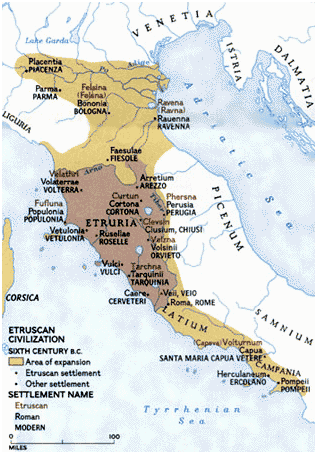
\includegraphics[width=0.7\linewidth]{../etruria}
\caption[Map of Etruscan territory]{Map of Etruscan territory}
\label{fig:etruria}
\end{figure}


\paragraph{}
As early as the 4th millennium B.C.E in Etruria, however, evidence shows that control over the production, distribution and consumption of resources was an important deciding factor in an individual's rank amongst his neighbors. Though there were few social divisions within these early societies, this practice of resource control was the basis for economic, political, and social competition which was the persistent driving force behind the process of their expansion. By the Late Bronze Age (1300-900 BCE) there was already significant intensification which lead to a shift from a landscape of only hamlets and farms to one that included, along with these, proto-urban villages. In this time period there was growth in the population with the appearance of new settlements, mostly on naturally defensible sites, valleys, and by major waterways. Expanded  territorial control fueled an increase in larger residences, hierarchical rankings, and economic activity with emphasis on animal secondary products, limited production of metals, and extensions of land use. While this time period still had a healthy population of inhabitants throughout the country it certainly marks the beginning of the process of nucleation and the formation of chiefdoms (44-59).

\paragraph{}  
Characterized by a dramatic increase in the process of nucleation, the Villanovan period (900-750 BCE), shows signs of further societal development.  Settlement numbers shrink considerably though those that prevail increase in population, size, and influence. Production and use of metals, especially iron, became indicators of wealth with much of the metals being obtained from key sources such as the Colline Metallifere, which translates to ``Metal-bearing hills'', or from the Tulfa Mountains \cite[75-77]{SpiSto92}. This is also the time period in which the first concrete evidence is recoded for habitation on the archaeological site of Poggio Civitate (Murlo). Located approximately 25km southeast of the Tuscan city of Siena on the eastern edge of the Colline Metillefere, this site shows three distinct phases of occupation on the plateau, Piano del Tesoro, of the hill. The earliest phase of occupation, the Iron Age (Coincides with Villanovan phase), is indicated by sparse remnants characteristic of pre-urban villages \citep{AnnAnd}.

\begin{figure}
\centering
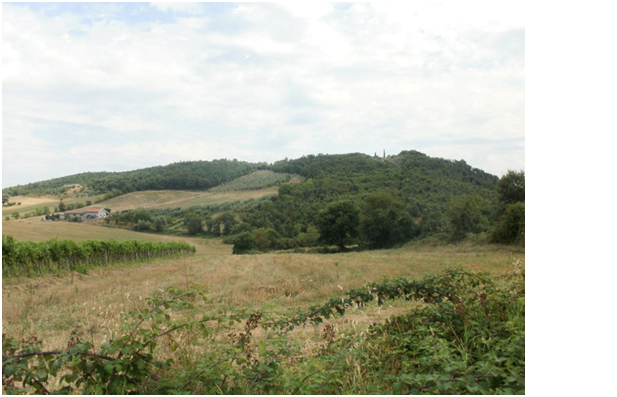
\includegraphics[width=0.7\linewidth]{../baseOfHill}
\caption{View of Poggio Civitate from the immediate periphery.}
\label{fig:baseOfHill}
\end{figure}

\paragraph{}
The later two phases of occupation differed in that they left behind significant archaeological remains of monumental architecture and are characterized by proto-urban traits such as craft specialization, social stratification, and increased consumption. The earlier of these two phases, starting in the 7th century BCE, consisted of three separate buildings (Figure \ref{fig:orientalizing}) each with a unique purpose: a tripartite building (three rooms) possibly for worship, a residence for an elite population, and a workshop for the manufacturing of bronze, bone, antler, ivory, food products, textiles, and architectural terracottas. A prolific burn layer in the soil stratigraphy along with unfired clay roofing tiles, which contained foot imprints, suggest that the site suffered from a sudden and fatal fire around 650 BCE. The plateau was subsequently scraped level and a new four-winged  complex (Figure \ref{fig:archaic}), approximately 60m in length each, was constructed (c. 600-580 BCE), which presumably incorporated all of the functions of the previous three buildings. Additional remains suggest the presence of watch towers and defensive walls that extended off of the main building. Unfortunately for the residents of the hilltop complex, it only survived a few decades before it was destroyed and abandoned between 550 and 535 BCE \cite[p. 35-45]{NieTuc01}

\begin{figure}
\centering
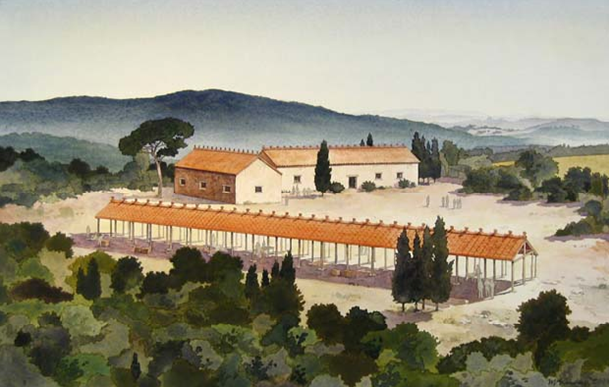
\includegraphics[width=0.7\linewidth]{../orientalizing}
\caption{Rendering of Orientalizing era (phase I) monumental architecture.}
\label{fig:orientalizing}
\end{figure}

\begin{figure}
\centering
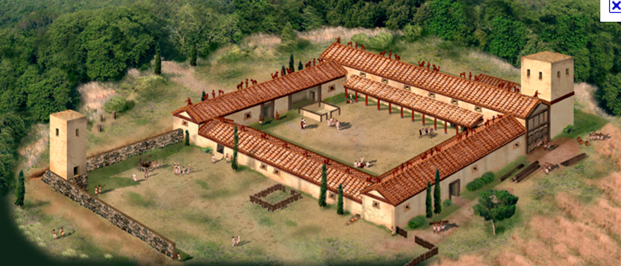
\includegraphics[width=0.7\linewidth]{../archaic}
\caption{Rendering of Archaic era (phase II) monumental architecture.}
\label{fig:archaic}
\end{figure}

\paragraph{}
While the exact reason for Poggio Civitate's eradication is unknown, the archaeological remains undeniably indicate that the occupants of the site commanded substantial authority.  The monumental architecture had rooftops adorned with captivating decorations (Figure \ref{fig:roof}) which would have been visible from afar and projected a message of social status to those at the site and within its periphery \citep{Tuc06,Odo13}. Additionally, the Archaic phase building featured a series of four recurring plaques displaying the lifestyle of an elite culture \cite[159]{Win09}. Due to a sudden destruction of the buildings, many items, normally considered portable, were left behind, including sets of elaborate bucchero cups, imported Greek vessels, large storage vessels, and hundreds of plates. This assemblage, which allows a glimpse into the society that dwelt on this hill, supports the theory that residents partook in banquets and feasts \cite[162-166]{BarRas98}. Material evidence signifies that those in control at Poggio Civitate likely dominated control over local natural resources and labor power. 

\begin{figure}
\centering
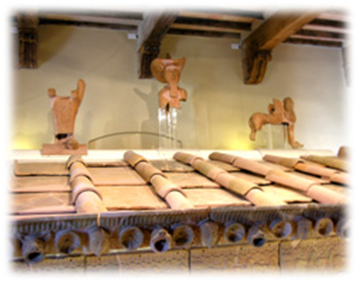
\includegraphics[width=0.7\linewidth]{../roof}
\caption{Rooftop decorations and statues.}
\label{fig:roof}
\end{figure}

\paragraph{}
Despite the status of the community at Poggio Civitate the site was not rebuilt after its destruction in the second half of the Sixth century BCE. In fact it was never reoccupied again and this seems to have been the intended goal of those responsible for the center's obliteration: as the walls were torn down the architectural terracottas were brought crashing to the ground. Some of the debris was then deliberately deposited in depressions throughout the site and covered with stone. The walls, along with soil and terracotta debris, were used to construct a mound, up to four meters high in some areas, along the perimeter of the plateau of Piano del Tesoro \citep{IEB94}. Additionally, roofing tiles were carried approximately 147.5m away from the Archaic phase building to intentionally seal a well that is speculated to have served a metal smelting industry or perhaps a residual community of Poggio Civitate \citep{TucBruHunTal10}. These actions maintain the theory that the destructors purposefully closed the hilltop site.

\paragraph{}
The permanent abandonment of the commanding hilltop of Poggio Civitate is surprising since modern civilization has proliferated on the crests of all other local hills. Many of these sites have in turn yielded archaeological remains from multiple eras \citep{Cam01}. It can be concluded that much of the landscape has been dotted with communities from ancient times until the present, except for Poggio Civitate.  After more than 40 years of excavations it is still unclear what forces caused residents to permanently vacate the hill's premises and why the hill was not resettled.

\paragraph{}
Everything that is known about Poggio Civitate, lacking formal reference in ancient texts, hails directly from the site's remains and the archaeologists who interpret them. Theories about why the settlement was destroyed or who the residents were must ultimately remain speculative. Modern literature produces a few prevailing, though vague, theories which attempt to answer questions about the origins and destruction of this elite civilization. 

\paragraph{}
Authors Barker and Rasmussen go as far as a general theory on the disappearance of Poggio Civitate. They explain that Murlo would have fallen into a category of medium-sized settlements that, due to their inland locations, were out of reach of the political authority of the larger cities. Though they would have initially developed autonomously, eventually these centers were abandoned or destroyed at a time when the major cities were growing in size and power. This is to say, simply, that these smaller centers were the ``losers'' in the process of urbanization and expansion. The authors distilled their theory out of the fact that Etruscan cities likely controlled extensive land beyond their city limits \cite[p. 100,176]{BarRas98}. As any municipality grew in size they would have needed to destroy opposition and maintain a network of governance to ensure hegemony in their territory. Barker and Rasmussen do not develop their speculation any further but from their ideas it is easy to imagine Poggio Civitate as a rival settlement where the inhabitants were overthrown by enemies. Setti and Bonamici \citeyearpar{SetBon85} posit that the settlement of Chiusi was relatively late in the urbanization process showing its first signs of aristocracy only by the end of the 7th century BCE, and displaying typical behavior of Etruscan cities by the mid-6th century. They list military control of the countryside and abandoning of the small scattered communities as two such indicators of the development process, similar to imagined scenarios based on Barker and Rasmussen's theory. Setti and Bonamici proceed by stating that Murlo, located on the border between Chiusi's and Rusellae's territory, was the first of many (Dolciano Sarteano, Cetona) communities to be abandoned. She pegs the rise of the Chuisian King, Porsenna, and the expansionist policy that he initiated to the approximate date of Poggio Civitate's abandonment in 525 BCE (32-33). Due to Murlo's centrality between the major cities of Volterra, Arezzo, Chiusi, Roselle, and Vetulonia, and the evidence for its ritual status, Edlund-Berry \citeyearpar{IEB94} argued that the site might have operated as a neutral meeting place for a confederation of these cities, under divine protection, until the confederation was abolished when Chiusi changed its political affiliation to the Tarquin dynasty at the end of the sixth century BCE \cite[p. 176-177]{BarRas98}.

\paragraph{}	
These various theories attempt to answer questions pertaining to Murlo though ultimately they are unable to provide evidence beyond a casual narrative.  Generally, they develop their theories by looking to the remains of the site itself or to that of another site to explain the series of events that define Murlo without considering the space between them. Aspatial, and sometimes site-centric approaches to collecting corroborating evidence or deducing theories, while useful, can be at a serious disadvantage for researching processes that occur at several scales over a large territory. This research is aimed at developing a more rigorous methodology that includes site-centric information but also includes a regional setting to test hypotheses pertaining to Murlo. More specifically, spatial interaction models will be deployed to test how Murlo's spatial attributes such as size and location would have defined its role in relation to other sites within the entirety of the Etruscan society.  The connectivity networks that result from the models will help to depict the developing Etruscan landscape and subsequently alleviate the mysteries surrounding Poggio Civitate.


\section{Spatial Interaction Theory In Archaeology and Within Etruria}

\paragraph{}
Interaction within regions seems to enjoy popularity as a theory of a driver for growth within civilizations \citetext{\citealp[226]{Kow08}; \citealp[380]{Bin83}}. Colin Renfrew \citeyearpar{Ren75} provides one of the most complete theories of interaction, in the form of trade, as a driver for the development of early states.  In this archaeological context he identifies examples of territories in which neighbors are modular central places defined  by evenly spaced settlements at about a 1500km square area and a mean distance of 40km to neighbors, although this latter measure has been shown to range from 20km to 100km (14). While Renfrew credits trade as the mechanism behind the spatial interaction, he also discusses how these interactions rely on the interdependence of material and spiritual aspects of human culture and inevitably leads to communication and information flows as well (4-5, 24-25). His argument is that habitual exchange leads to central places since it requires organization and security and it implies some assumed criteria of value. He is careful to insist, however, that central places do not necessarily require civilization, but that they inevitably result in some form of interaction amongst those within the nucleated settlement (6-7). Ultimately, these central places provide a wealth of benefits in the form of market efficiency, as well as forums for solidarity and conflict resolution.  Competing centers result in more specialization that will further demand for the trade of goods between central places thus promoting greater interaction (9-10, 26-29).

\paragraph{}	
According to Renfrew, trade can be broken down into different categories,  including extra-regional trade, internal trade within a settlement's domain and trade between these domains within a region.  It is this last form of trade that Renfrew claims is the least studied despite the idea that its ``effect must have been to produce and maintain the uniformity of culture or civilization as a whole'' (18). He also states that ``Civilization implies the development of a highly structured and differentiated society, with specialist production (craftsmen), a permanent controlling organization disposing of a significant proportion of produce (government), and a developed, explicit set of shared beliefs (cognitive structure), sometimes with large aggregations of population'' (35). This suggests that those sites which have remains indicative of increasingly civilized characteristics would have likely participated in more inter-site trade amongst the larger central places. Similarly, Izzet cites increased encounters with ``others'' as a driving factor in attitude changes towards ethnic identity. In this process, the differentiation of the self is an effect which takes place only after  discovering ``others'' (2007, 210) . Physical growth and cultural development are therefore inextricably linked and, to a certain degree, controlled through the common process of interacting through space. 

\paragraph{}
It is difficult to differentiate between interaction and the growth of civilization. For example, population increases, which may have resulted from market benefits gained through trade and interaction, would have been likely to cause squabbles over territory. Tension amongst regions would initiate contact as well as competition which results in greater cultural development as well as further interaction (234). In contrast, the process of state emergence can be envisioned from the standpoint of external trade \citep{Pen11} using the Kipp-Schortmann model. This model holds that when a state society initiates contact with a chiefdom society, the elites of the latter, who will likely be sole recipients of the initial exchange, will experience an increase in power through the acquisition of new prestige goods. To maintain their authority over access to the new commodities the elites will resort to violating social norms which eventually erodes their legitimacy.  From the collapse of their power emerges the new organization of the state (181-183). Pena admits that his application of this model within Etruria produces pessimistic conclusions (196). Interestingly, he doesn't even consider internal trade as the mechanism that leads to the formation of states within Etruria. It is easy, however, to envisage this process occurring between social groups with differing ranks within a hierarchical structure without even incorporating external groups. If prestige is gained from trade goods that originate from farther away, more prestigious places then it is evident that distance played an important factor in the development of the involved societies. While it is still difficult to prove that this concept directly lead to more complex civilization it does nicely portray the importance on spatial contexts within Etruria which is able to provide a strong theoretical framework for measuring interactions amongst different groups. 

\section{Modern Transportation Geographic Theory}

\paragraph{}
Modern geographic theory pertaining to transportation studies is largely in agreement with the theories that have been developed within archaeology and are therefore helpful in providing a supporting theoretical framework for spatial interaction modeling. At the root of transportation theory lies the idea of complementarity which holds that different locations must have varying surpluses and deficits in order for the exchange of goods, ideas or people to occur (Comtois, Rodrigue, and Slack, 2006, 7). The ensuing interactions are further conditioned by environmental factors such as topography, hydrography, and climate. For example, transportation has historically followed paths along plains, valleys, and mountain passes while avoiding physical impediments. Similarly, available waterways, ports, access to natural resources and severe weather have been major considerations within transportation systems (8). What each of these factors have in common is that they incur a cost which must be considered against the benefits of carrying out the proposed transportation. Clearly, the spatial structure of the resulting transport network is a product of these environmental factors along with properties at each location which facilitate the creation of supply and demand and therefore affect the associated costs. In archaeology the decision process of whether or not to interact and subsequently travel from one site to another would have involved the same factors so that the derived spatial structure of an interaction network would be subject to the same constraints.    

\paragraph{}
	
The accessibility, or the measure of a site's ability to reach or be reached by another site, is a product of the established spatial structure. Distance, which is often measured by cost, is inversely proportional so that more accessible sites tend to be closer together, have less associated costs and are deemed more valuable. Agglomeration and specialization of activities is likely to take place at more valuable locations to reduce transportation costs and therefore further increase the value of a location. A location specializing in a commodity or activity may also drive segregation between itself and other locations as a side effect. In the process of transportation development, two forces are constantly in effect: concentration and dispersion. Coupled with the fact that transportation systems are subjected to the constraints of historical spatial structures it is apparent that these networks are highly dynamic yet they are constantly being conditioned (11-28). Typically the networks evolve to increase efficiency, decrease costs, and increase accessibility. Archaeological interaction networks would have been under similar influences making their development equally as dynamic. It is also therefore possible to assume that a proposed interaction network based on physical attributes should approach an approximate maximum efficiency and accessibility. Given the complexities within transportation geography and the overlap in theory with ancient interaction networks it seems appropriate to employ modern analytical methods within archaeological contexts.



\section{Spatial Interaction Theory and Modeling}

\paragraph{}
Spatial interaction encompasses an array of behaviors, such as communication or movement which occur over geographic space as a result of a decision process \citep[1]{FotOke89}. Its broad definition has allowed it to support a diversity of research within migration, shopping, recreation, commodity and capital flows, communication, transportation networks, and commuting (Haynes AND Fotheringham, 1984). In each application a trade-off is considered between the benefits accrued through interaction versus the costs necessary to traverse space to carry out the interaction. By encoding spatial interaction into a mathematical model it is possible to explain an observed phenomena or to use observed data in order to make predictions about the future or alternative scenarios \citep[2]{FotOke89}. This is particularly useful in circumstances where the number of locations under consideration or the factors involved in the decision-making process are large. Typically the interaction can be summarized by a matrix in which each row, $i$,  represents a possible origin and each column, $j$, represents a possible destination. As a result the interaction between any two locations can be described by flow $ij$ and the total interaction in or out of a site can be found by summing a row or column.    
	
\paragraph{}
Earliest spatial interaction models were developed using an analogy to gravitational forces from the field of physics (Roy AND Thill, 2004, 2). The Newtonian gravity model is relatively simple:\\
				\begin{equation}
				T_{ij} = \frac{k(P_{i}*P_{j})}{D_{ij}}
				\label{eq:simpleGrav}
				\end{equation}
				
where $T_{ij}$ denotes the aggregate flow between origin $i$ and destination $j$, $P_{i}$ and $P_{j}$ represent the size, population, or density of the origin and destination, and $D_{ij}$ is the physical separation between these two locations. It is apparent that given fixed values of $P_{i}$ and $P_{j}$, as $D_{ij}$ is increased, the value for $T_{ij}$ will decrease, therefore accounting for the costs of overcoming further distances. Additional parameters were later added to reflect the relationship of spatial flows and explanatory variables \cite[216]{FotBruCha02} which allowed customization of the model for different applications.  The gravity model faced criticism for its lack of theoretical foundations despite the fact that it produced reasonably accurate estimates of spatial flows (217).  A more stable theoretical grounding was developed in the 1960's by the work of retail modelers and regional planners \cite[2]{RoyThi04}. In the 1970's Wilson introduced a new framework for interaction modeling which relied on maximizing the entropy of the flow system. An aggregate flow between two locations is considered a macro state which can be satisfied by various micro states. The fundamental principle in entropy-maximizing models is that the most likely macro state is one which can be described by the highest number of micro states \cite[17-19]{FotBruCha02}. Adding in constraints allows for the derivations of a family of models in which information about origins, destinations, or both can be added to the model before solving for the most likely state \cite[4]{Wil10}. Despite the analytical gains of the maximum entropy models, criticisms arose due to the fact that it was still based on a physical analogy and that many of the applications lacked a behavioral interpretation \citep{Oke04}.

\paragraph{}	
Consequently, more contemporary efforts in the development of spatial interaction modeling has been to derive models based on spatial information processing. Fotheringham \citeyearpar{Fot83} developed the competing destinations model to accommodate the fact that during the decision-making process an individual will be faced with a unique spatial distribution of alternative locations for every destination under consideration. The competing destinations model incorporates the fact that individuals do not always consider every other location. The attributes of each alternative can contribute to how and whether or not an individual considers it at all. As a result, it is entirely possible for decisions to be made that do not reflect maximum utility since they may not even evaluate every possible choice. More recently, Simini, Gonzalez, Maritan, and Barabasi \citeyearpar{Bar12} present the radiation model as an entirely new framework which deviates from the gravity law concept which has been at the core of most previous models. The authors assert that their model overcomes no fewer than six known limitations of some previous gravity law models, most notably of all is that the model is parameter free and therefore requires no previous flow data for calibration. They also claim that their model permits a lack of interaction to have a priority over benefits gained in interacting. For  each possible origin and destination pair, flows are predicted by comparing the benefits of interacting with one proposed destination to the benefits of interacting with each other site within a radius from the origin equal to the distance from the origin to the proposed destination. Formally, these flows are given by the following,
			
				\begin{equation}
				T_{ij} = T_{i}\frac{(M_{i}*N_{j})}{(M_{i}+S_{ij})(M_{i}+N_{j}+S_{ij})}
				\label{eq:originalRad}
				\end{equation}
				
where $T_{ij}$ represents the flow prediction, $M_{i}$ and $N_{j}$ are density measures (e.g. population or size of a settlement) of the origin and destination respectively, $S_{ij}$ is the total density of all other alternative locations, and $T_{i}$ is a scaling factor that represents a proportion of the total number of commuters starting at a location which serves to ensure that commuter flows are not larger than the origin population.  Thus the model depends not directly on the distance variable but rather the aggregate benefits (e.g. population of a city) available at all other alternative choices between the origin and destination lending itself to the analogy of radiation and absorption processes (1-2). 

\paragraph{}	
Performance of the radiation model's over the simple gravity model in a wide range of applications and scenarios (hourly mobility, daily commuting, yearly migrations is allegedly superior over basic gravity models (4-5, figure 3). Therefore, given the simplicity of the radiation model and its proposed gains in analytical accuracy, it will be chosen as one of the three models proposed for this research. In the context of ancient spatial interaction $M_{i}$ and $N_{j}$ will be given by a proxy for population (e.g. urban area) which will provide a relative measure of populations throughout the study region. At present, there is no known research in which this model has been employed in the field of archaeology, which will provide an interesting comparison to past work that is founded upon the gravity law and distance decay.

\section{Spatial Interaction Modeling in Classical Archaeology}

\paragraph{}	
Renfrew and Level's XTENT model \citeyearpar{RenLev79} was an attempt to model the effects of space within an archaeological region using a stronger theoretical framework. The model, which is based upon Renfrew's previously discussed (section 2.2)  theory of trade and statehood, was designed to divide territory between respective central places and is defined by six  axioms (145-146):

	
\begin{enumerate}
\item The human social group is defined by the habitual association of persons with a territory
\item Human organization is segmentary in nature: human spatial organization is therefore cellular and modular.
\item Basic social groups do not exist in isolation, but affiliate together into larger groups, meeting together at periodic intervals. 
\item Human society is often hierarchical in nature: Human spatial organization is therefore 	stratified.
\item The effective polity, the highest order of social unit, may be identified by the scale and 	distribution of central places.
\item Special interactions between polities undoubtedly take place, creating uniformities in 	artifact distribution: Such uniformities in themselves do not document societies or people.
\end{enumerate}

\paragraph{}
Following these lines of thought, we can conclude that a) within social groups people will periodically interact giving rise to meeting places, b) human societies are often hierarchical  which necessarily implies a spatial patterning, and c) between these social groups or polities there is interaction. They are sure to note that the distribution of artifacts due to these interactions, which would become more uniform with increased  exchange, would be less indicative of individual societies. This can be interpreted as warning against the perils of using objects as a proxy for populations and their interactions in certain contexts as opposed to geographic features such as urban extent. The authors admit that their theory gives rise to their own version of Central Place Theory though they maintain that it is different than Christaller's Central Place Theory of economic man (146). Ultimately, his model describes hierarchy through competition rather than evaluating how space mediated interaction within settlement networks. For this reason, the model will not be used in this research which seeks to directly compare relative spatial interaction; however, Stoddard and Redhouse's \citeyearpar{StoRed11} extension of the XTENT model to Etruria (Figure \ref{fig:stoddard}) provides insight into territorial dynamics of the region under inspection. They conclude that Poggio Civitate would have initially existed as an autonomous entity outside the of reach of larger settlements. Eventual expansion and competition resulted in its absorption (168-169), strongly agreeing with the arguments previously explained (section 2.1). Their interpretations are useful for the comparison of models results presented in later sections of this research. 

\begin{figure}
\centering
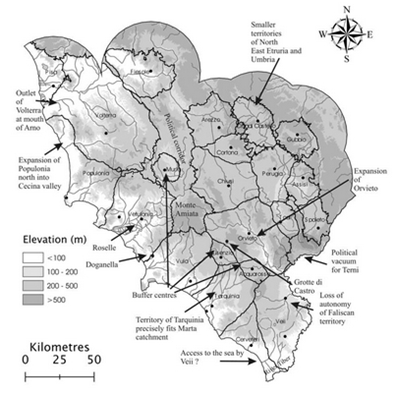
\includegraphics[width=0.7\linewidth]{../stoddard}
\caption{Results from the XTENT model for Etruria.}
\label{fig:stoddard}
\end{figure}

\paragraph{}
A simple model which has been employed in archaeology \citep{Bro00} for measuring connectivity is proximal point analysis (PPA). In PPA each site is connected to its $K$ nearest neighbors (constant value set by user) so that distance is not considered in the decision making process. In contrast, a maximum distance network (MDN) considers two sites connected if the distance between them is less than model parameter D, (constant value set by the user). Both models are inherently prohibitive, MDN's in that any site beyond the set distance is eliminated from the network and PPA in that a site may only maintain a limited number of links \cite[5-10]{ERK12}. One defining limitation of PPA approach is that all sites must participate thus forcing even the farthest sites to connect somewhere despite being potentially isolated. In a sense, both of these models are unrealistic because they only account for a limited set of scenarios. It is possible that sites close in proximity never visited each other due to resource sufficiency or  that communities located miles away still benefited from interaction regardless of distance and as a result made long journeys. Additionally, these simple models do not designate flow directions for the links; either two sites are simply connected or they are not which excludes the option for non-reciprocal relationships. The simplicity of these models makes them easy to apply but leaves many open questions during analysis.

\paragraph{}	
Gravity models were  adopted by David Clarke, a prominent spatial theorist within archaeology, who was a proponent of quantitative methods in the late 1960's and 1970's. In Analytical Archaeology he took a systemic and model approach to explain patterns in culture, technology, and the environment \citep{Cla68} and later in Spatial Archaeology \citep{Cla77}  he tackled issues of scale and space directly along with several additional authors who examined settlement structures, land use patterns and simulated the spread of settlements. This type of work was subjected  to the typical critiques of early quantitative methods. It was believed that  they over looked true social theory and that the anthropological neutrality claimed by these methods was actually biased towards the scientists employing them \cite[72]{Hod03}.

\paragraph{}
Building on previous work with gravity models Rhil and Wilson \citeyearpar{RihWil91} employ maximum entropy principles to simulate settlement patterns in Geometric mainland Greece. They ask the question, ``Did location vis-a-vis other settlements have a significant effect on their affiliation and union?'' (61). They argue that it is sufficient to use ``as the crow flies'' straight lines despite lacking a true representation of Greece's rugged terrain because this information would have been incorporated in the dataset through settlements pre-determined locations and density. While they claim this assumption yields effective results it ignores the fact that settlement location selection and travel preferences constitute two different actions. A site may have been initially established for defense or proximity to resources without consideration or even any knowledge of many other site locations. Another important detail in Rhil and Wilson's model is that all sites start off with the same size and importance due to what they call the ``egalitarian hypothesis'' and these attributes are then predicted as part of the model. Validation is therefore possible between the model results and the attributes measured from the archaeological record. Two additional parameters, the benefits of concentrated resources and the difficulty of communication, enable the model to be fine tuned.   Their work offers an improvement on simple geographic models and elementary gravity models in archaeology by adding constraints and parameters, though it is not without flaws.  One limitation is that the model inherently creates networks that are ``supply side''. This means that larger cities attract the interactions of the nearest smaller sites, never allowing small sites to connect with each other. In effect, you get a network reminiscent of a star pattern (Figure \ref{fig:rhilWilson}) which is helpful for identifying key nodes but still may not represent a realistic network. Their gravity model also lacks the ability to capture the feedback effects of interactions and site size on each other \cite[10]{KnaEvaRiv08}.

\begin{figure}
\centering
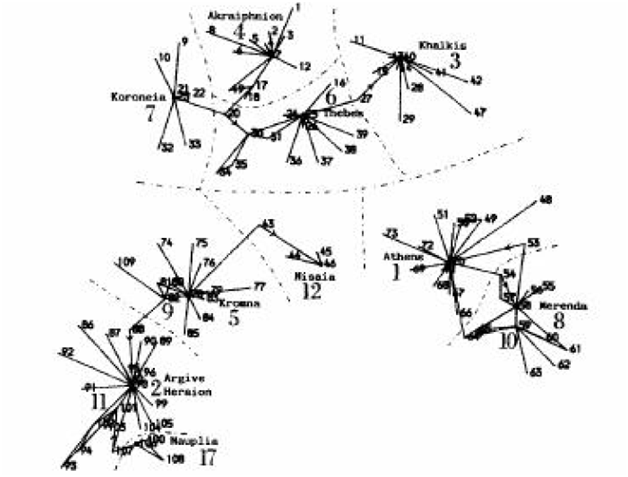
\includegraphics[width=0.7\linewidth]{../rhilWilson}
\caption{Results from Rhil and Wilson's maximum entropy gravity model.}
\label{fig:rhilWilson}
\end{figure}

\paragraph{}
Ariadne, the model developed by Evans et al., is a type of gravity model that has improved upon the work of Rhil and Wilson. They employ a ``Hamiltonian'' energy function, H, consisting of four terms, which takes the form,
			\begin{equation}
			H = -kR - \lambda E + jP + \mu T
			\label{eq:simpleHam}
			\end{equation}  
where $R$ is the benefits of exploiting local resources, $E$ is the benefits of maintaining links, $P$ is the cost of supporting local populations and $T$ is the cost of maintaining links. Each term has a parameter which controls the effect it has within the model. Expanding the terms give $H$ the following form,
			\begin{equation}
			H = -k\sum_{i}S_{i}v_{i}(1-v_{i}) - \lambda\sum_{i,j}V(\frac{d_{ij}}{D})\cdot(S_{i}v_{i})\cdot e_{ij}\cdot (S_{j}e_{j}) + j\sum_{i}S_{i}v_{i} + \mu\sum_{i,j}S_{i}v_{i}e_{ij}
			\label{eq:expandedHam}
			\end{equation}

where $S_{i}$ is the given size of a site, $v_{i}$ and $e_{ij}$ are outputs of the model representative of the weight of each settlement and interaction link in the network, and $V(\frac{d_{ij}}{D})$ provides a gravity function based on the distance between two nodes ($d_{ij}$) and an average maximum journey length ($D$). $H$ provides a tool for balancing the cost and benefits of both ``supply'' and ``demand'' between site interactions. Using optimization techniques a minimum value is obtained for $H$ and the model output values ($v_{i}$ and $e_{ij}$) can be read off and visualized as a network (10-24). 

\paragraph{}
The additional output of interaction ``strength'' ($e_{ij}$) makes it possible to create a network in which all nodes participate yet closer sites will have strong links and farther sites will have weaker ones. It is also feasible that some sites may choose not to interact because their costs outweigh the benefits. Unlike Rhil and Wilson, smaller neighbors are free to interact with each other rather than being limited to the hierarchical ``star'' pattern. Ariadne is also superior because it incorporates ``course-graining'', the assumption that the whole is the sum of the parts, meaning that one value can be used to represent the exchange departing or arriving from multiple sites if they exist within a very close proximity. In archaeology this is crucial in supporting sometimes incomplete and ambiguous records for local regions. An important feature of the Ariadne model is that it is stochastic rather than deterministic. Each model run yields slightly different results which approach some optimal solution therefore mimicking short-term fluctuations within the system. A comparison of multiple runs allows the isolation of a most likely optimal solution \citep[12]{ERK12}. Due to Ariadne's abundance of advantages and ability to produce the most realistic settlement networks, it will be selected as the second model to simulate network interactions in central Italy. Ariadne's later deployment to investigate the effects of the destruction of a central node in the Greek maritime network as a result of the volcanic eruption of Thera \citep{KnaRivEva11} is directly comparable to the study of Poggio Civitate and its disappearance. Analysis in this research will therefore draw heavily from the methodology of Evans, Knappet, and Rivers.
	
\paragraph{}
Model three, inspired by the TravellerSim model, introduces an entirely new modeling framework into this research while still building off the work of by Rhil and Wilson. Graham and Steiner \citeyearpar{GraSte08} propose a method for observing the emergence of territories from the perspective of the individual. The general motivation for this agent-based approach is that it is not truly possible to know the exact relationship between sub-systems within a larger system. Instead we can assign very simple rules to individuals and then let them interact, thus developing the more complex relationships observed at the macro level. TravellerSim is built upon the same assumptions put forth by Rhil and Wilson \citep[64, 71]{RihWil91}, except spatial decisions are now limited to a local vision (approximately 20km from the settlement the agent is currently at). Each round, the agents consider 3 settlements within their vision and then choose to travel to the most ``attractive'' destination. Attractiveness is calculated using a localized version of Rhil and Wilson's equation:

		\begin{equation}
	 	A = \frac{importance^{\alpha} * e^{-\beta D}}{visitors^{\alpha} * e^{-\beta D}}
		\label{eq:attractiveness}
		\end{equation}
	
where the importance is the current importance of a site, $\alpha$ is a parameter to represent the benefits from resources, $\beta$ is a parameter to represent the cost of communicating over space, and $D$ is the distance from the agent to the settlement whose attractiveness is being calculated. After all agents have moved settlements then update their importance based on the interaction they received following:

		\begin{equation}
	 	New Importance = V * \sqrt{\frac{\sum{I}}{v}} 
		\label{eq:importance}
		\end{equation}
 
where the $V$ is the cumulative total number of visitors who has arrived at a settlement, $I$ is the importance values from each of the settlements an arriving agent had originated for a given iteration, and $v$ is the number of visitors at each settlement for the current round. 

\paragraph{}
In this manner the authors were able to successfully ``grow'' fuzzy territories and visualize the spread of influences over the region. Furthermore, by tracking the individual visits of the agents it is possible to visualize a weighted directed network similar to the Radiation model and Ariadne. In this respect, TravellerSim is not limited like Rhil and Wilson's model or the XTENT model despite their shared interest in hierarchy and territory. Overall, the bottom-up approach demonstrated in TravellerSim contributes a solid base on which to develop an interesting alternative to the more top-down concepts employed in the other two models selected for this research and will therefore be selected as the third model to study spatial interaction patterns within ancient Etruria. 

\chapter{Problem Statement and Hypothesis}

\paragraph{}
It is apparent from the literature (section 2.1) that there are two main theories which assume differing relationships over space. By defining the inherent inter-settlement associations, or lack thereof, that would have been present in each scenario we can develop tests to evaluate them. Our primary question, therefore, is ``was Murlo an autonomous central place or did it feed into a larger hierarchy of settlements?''. We can then propose the following simplified theories from the literature on the nature of Poggio Civitate:
	
	\begin{enumerate}
	\item Murlo was a relatively autonomous settlement which enjoyed independence from the influence and authority of other central places despite its relatively smaller size.
	\item Murlo acted as central meeting place for the other Etruscan powers to meet in a neutral setting due to its central location to other settlements. 
	\end{enumerate}

\paragraph{}
To test these theories we need to embed Murlo into an interaction network with other contemporary sites. Theory one suggests that Murlo would have engaged in very little interaction given its location and size. More importantly, we must differentiate between incoming and outgoing interaction. For Murlo to remain autonomous we would expect relatively little incoming traffic since it was not subject to the influence of other settlements. Therefore, limited overall interaction will provide evidence for theory one though some outgoing interactions with minimal incoming interaction would still be considerably strong evidence. Conversely, theory two assumes strong interaction predictions amongst Murlo and its surrounding neighbors, especially in terms of incoming traffic. This is not to say that Murlo's neighbors would not have also interacted strongly with each other in their regular affairs. Rather, these interactions will be used as the base for a comparison to associations with Poggio Civitate.

\paragraph{}
Another objective of this research is to use a geographical approach to determine how the destruction of Poggio Civitate factored into the dynamics of the larger system. Unfortunately, the spatial distribution of settlements does not directly provide information on the demise of Murlo. Instead, we can use the quantitative models to simulate interaction networks with and without Murlo in order to answer the question, ``How did the destruction of Poggio Civitate effect the strength and distribution of interaction throughout the wider region of Etruria?''. If the network remains relatively unchanged it will count as evidence towards Murlo as an autonomous central place. Likewise, if we record large shifts in the network we can conclude that it is likely that Poggio Civitate was playing an important role in the wider region of Etruria and that its destruction may have been related to its favorable location. 

\chapter{Methodology}
\section{Data}

\paragraph{}
For all of the chosen models, the only necessary data is a selection of settlements, their geographic coordinates, a proxy for each site's population or size, and a measurement of distance between all pairs of sites. Considering Renfrew's warning against relying on artifact counts and the unavailability of population estimates, the urban extent of a site's archaeological remains will be used to represent its size. Settlements taken into consideration (figure \ref{fig:Sites}) for this research are those used by Stoddart and Redhouse (2011) to test the Early State Module concept of Colin Renfew (1975). Under Renfrew's theory, the characteristics of early state societies included autonomous central places,  a uniform spacing of about 40km amongst neighbors, approximately 1500 square kilometers of territory per polis, and the region consisted of a cluster of about a dozen sites. Stoddart and Redhouse (2011) provide a list of 25 Etruscan settlements and their corresponding size estimates which co-existed in time period roughly from 900 to 600 BCE. Though their research shows that only a fraction of the sites ultimately meet the ESM standards using the XTENT model, we can nevertheless adopt their study sites for use in our spatial interaction models given that this research has no restriction to solely early states. Their data provides the best available starting point for spatial interaction modeling in this context because they have assembled site size estimates by drawing from various archaeological sources as well as personal experience when no estimation existed (166). Following Stoddart and Redhouse, the sites, as presented in Figure \ref{fig:SiteData}, were all given spatial context via the Latitude and Longitude attributes from the Getty Thesaurus of Geographic Names Online with the exception of Bisenszio. Each site's name was queried in the on-line thesaurus, and if an entry existed for the ancient site as opposed to the modern one, then it was used. If only one entry existed (modern or ancient), then it was utilized. For Bisenzio, which was not listed in the thesaurus, coordinates were estimated visually using its known location via Google Earth. Finally, each settlement's coordinates were transformed using the Web Mercator Auxillary Sphere projection and the WGS1984 datum (EPSG: 3857), in order to perform geo-computation within a GIS.

\begin{figure}
\centering
\includegraphics[width=0.7\linewidth]{../Sites}
\caption{Study sites within their natural topographic (elevation) environment.}
\label{fig:Sites}
\end{figure}


\begin{figure}
\centering
\begin{tabular}{|c|c|c|c|c|}
\hline \textbf{Name} & \textbf{Number} & \textbf{Size (ha)} & \textbf{GettyLon} & \textbf{GettyLat} \\ 
\hline 	Veii	&	1	&	185	&	42.0333	&	12.4	\\
\hline 	Cerveteri	&	2	&	160	&	42	&	12.1	\\
\hline 	Vetulonia	&	3	&	100	&	42.85	&	10.9667	\\
\hline 	Populonia	&	4	&	150	&	42.9833	&	10.4833	\\
\hline 	Volterra	&	5	&	100	&	43.4	&	10.85	\\
\hline 	Chiusi	&	6	&	50	&	43.0167	&	11.95	\\
\hline 	Bisenzio	&	7	&	35	&	42.57	&	11.87	\\
\hline 	Acquarossa	&	8	&	30	&	42.4833	&	12.1333	\\
\hline 	Perugia	&	9	&	32	&	43.1333	&	12.3667	\\
\hline 	Gravisca	&	10	&	24	&	42.2	&	11.7167	\\
\hline 	Gubbio	&	11	&	20	&	43.35	&	12.5833	\\
\hline 	Assisi	&	12	&	20	&	43.0667	&	12.6167	\\
\hline 	Citta di Castello	&	13	&	20	&	43.45	&	12.2333	\\
\hline 	Tarquinia	&	14	&	150	&	42.25	&	11.75	\\
\hline 	Vulci	&	15	&	126	&	42.4167	&	11.5833	\\
\hline 	Roselle	&	16	&	40	&	42.8	&	11.1333	\\
\hline 	Murlo	&	17	&	10	&	43.15	&	11.3833	\\
\hline 	Pisa	&	18	&	20	&	43.7167	&	10.3833	\\
\hline 	Orvieto	&	19	&	85	&	42.7167	&	12.1167	\\
\hline 	Arezzo	&	20	&	32	&	43.4167	&	11.8833	\\
\hline 	Cortona	&	21	&	30	&	43.2667	&	11.9833	\\
\hline 	Civita Castellano	&	22	&	26	&	42.2833	&	12.4167	\\
\hline 	Fiesole	&	23	&	30	&	43.8	&	11.2833	\\
\hline 	Todi	&	24	&	20	&	42.7833	&	12.4	\\
\hline 	Spoleto	&	25	&	20	&	42.7333	&	12.7333	\\
\hline
\end{tabular} 
\caption{Sites used in the study and their attributes.}
\label{fig:SiteData}
\end{figure}

 
\paragraph{}
It is important to note the possible boundary effects that might arise from this data set. While this list includes the significant settlements that existed throughout the time period of interest there would have undeniably been considerable interaction occurring between sites within the study region and those external to it, especially for those settlements close to the study region border. This is a problem that will arise at any scale and for any study region. Regardless, we must limit the boundaries in order to maintain conceptual simplicity as well as managing computing resources.  
	
\paragraph{}
Many  methods are available for obtaining inter-settlement distances. Straight line or ``as the crow flies'' distance is the simplest measurement to employ since it requires no abstract concept of cost and can be easily computed using Euclidean distance calculations. It is obvious, however, that most network edges cannot be truly represented without incorporating the natural terrain. Bevan \citeyearpar{BevForthcoming} reviews several alternate methods that have been deployed by archaeologists to integrate the landscape into distance calculations. Arguably an entire study could be completed solely on choosing a proper representation of travel times or costs over space. As a compromise, this research will leverage methods similar to those utilized by Stoddart and Redhouse (165) within the XTENT model whenever possible. This will promote consistency, incorporate the effects of the terrain, and  maintain simple and reproducible calculations. Ultimately, though, the method employed here must differ since this research seeks to incorporate the terrain by deriving least accumulated cost paths between sites whereas Stoddart and Redhouse aimed to create cost distance rasters for the entire region.

\paragraph{}	
Distances between sites will be reflective of the least accumulated path given the energy costs ($J\cdot kg^{-1}\cdot m^{-1}$) necessary to traverse natural slopes within the terrain. To carry out this calculation an ASTER 30m resolution digital elevation model will be used to derive the slope of the terrain, which is an improvement in resolution over previous research \citep[165]{StoRed11}. The elevation DEM was clipped (figure \ref{fig:Sites}) to a buffer of two times the average nearest neighbor distance (straight line) of the settlements and to the natural coast line of the Italian peninsula (167). A slope raster was then calculated with the clipped DEM as the input. Differing ``costs'' to travel from one site to another were computed by classifying each slope raster cell by the associated required energy to traverse it as proposed by Stoddard and Redhouse \citeyearpar{StoRed11}. Data for the average cost of walking and cost of running for slopes ranging from -45 to +45 degrees \citep{Min02} is given in figure \ref{fig:CostData}.   

\begin{figure}
\centering
\begin{tabular}{|c|c|c|}
\hline Slope & Cost of Walking & Cost of Running \\ 
\hline -45 & 3.46 & 3.92 \\ 
\hline -40 & 3.23 & 3.49 \\ 
\hline -35 & 2.65 & 2.81 \\ 
\hline -30 & 2.18 & 2.43 \\ 
\hline -20 & 1.3 & 1.73 \\ 
\hline -10 & 0.81 & 1.93 \\ 
\hline 0 & 1.64 & 3.4 \\ 
\hline 10 & 4.68 & 5.77 \\ 
\hline 20 & 8.07 & 8.92 \\ 
\hline 30 & 11.29 & 12.52 \\ 
\hline 35 & 12.72 & 14.43 \\ 
\hline 40 & 14.75 & 16.83 \\ 
\hline 45 & 17.33 & 18.93 \\ 
\hline 
\end{tabular} 
\caption{Energy cost of walking and running on different slopes ($J\cdot kg^{-1}\cdot m^{-1}$).}
\label{fig:CostData}
\end{figure}

\begin{figure}
\centering
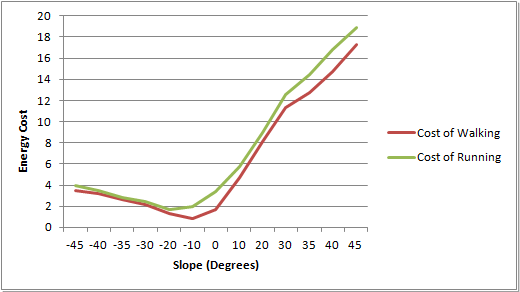
\includegraphics[width=0.7\linewidth]{../EnergyCostData}
\caption{Direct relationship between cost and positive slopes for both walking and running.}
\label{fig:EnergyCostData}
\end{figure}



Since the distances between the sites are long enough to prohibit an average person from running the entire trip only the values for the cost of walking were considered. It should also be noted that for most slopes the cost of running is not much higher than walking and that both actions follow a similar increasing trend (figure \ref{fig:EnergyCostData}). Additionally, the least accumulated cost path does not consider whether the slope is uphill or downhill. Since it is impossible to incorporate the costs of traversing both positive and negative terrain only the costs associated with positive slopes will be used to classify the slope raster due to the more prohibitive costs associated with traveling up hill. 

\begin{figure}
\centering
\begin{tabular}{|c|c|}
\hline Slope Range & Cost Classification \\ 
\hline 0-10 & 1 \\ 
\hline 11-20 & 2 \\ 
\hline 21-35 & 3 \\ 
\hline 36-45 & 4 \\ 
\hline 46+ & 5 \\ 
\hline 
\end{tabular} 
\caption{Cost classification for each slope range.}
\label{fig:slopeClass}
\end{figure}

Given the following assumptions, a general cost class was assigned to each slope range (figure \ref{fig:slopeClass}) to produce a cost or friction raster which was used as input to derive the least accumulated cost paths in origin-destination matrix format \citep{Eth11}. These calculated values (Appendix Table \ref{fig:LCP}) are all longer than the straight-line distances (Appendix Table \ref{fig:crowDist}) since they tend to closely gravitate towards areas with lower slopes. They represent the route which will require the least energy to be exerted without greatly deviating from the shortest possible path. Developing a distance measurement that is representative of a physical transportation network preserves the network's edges length units which enhances the ease with which the model results can be interpreted. Additionally, a non-abstract measure of distance preserves the ability of the data to be verified against both contemporary knowledge and future discoveries of ancient roads within the study region.

\begin{figure}
\centering
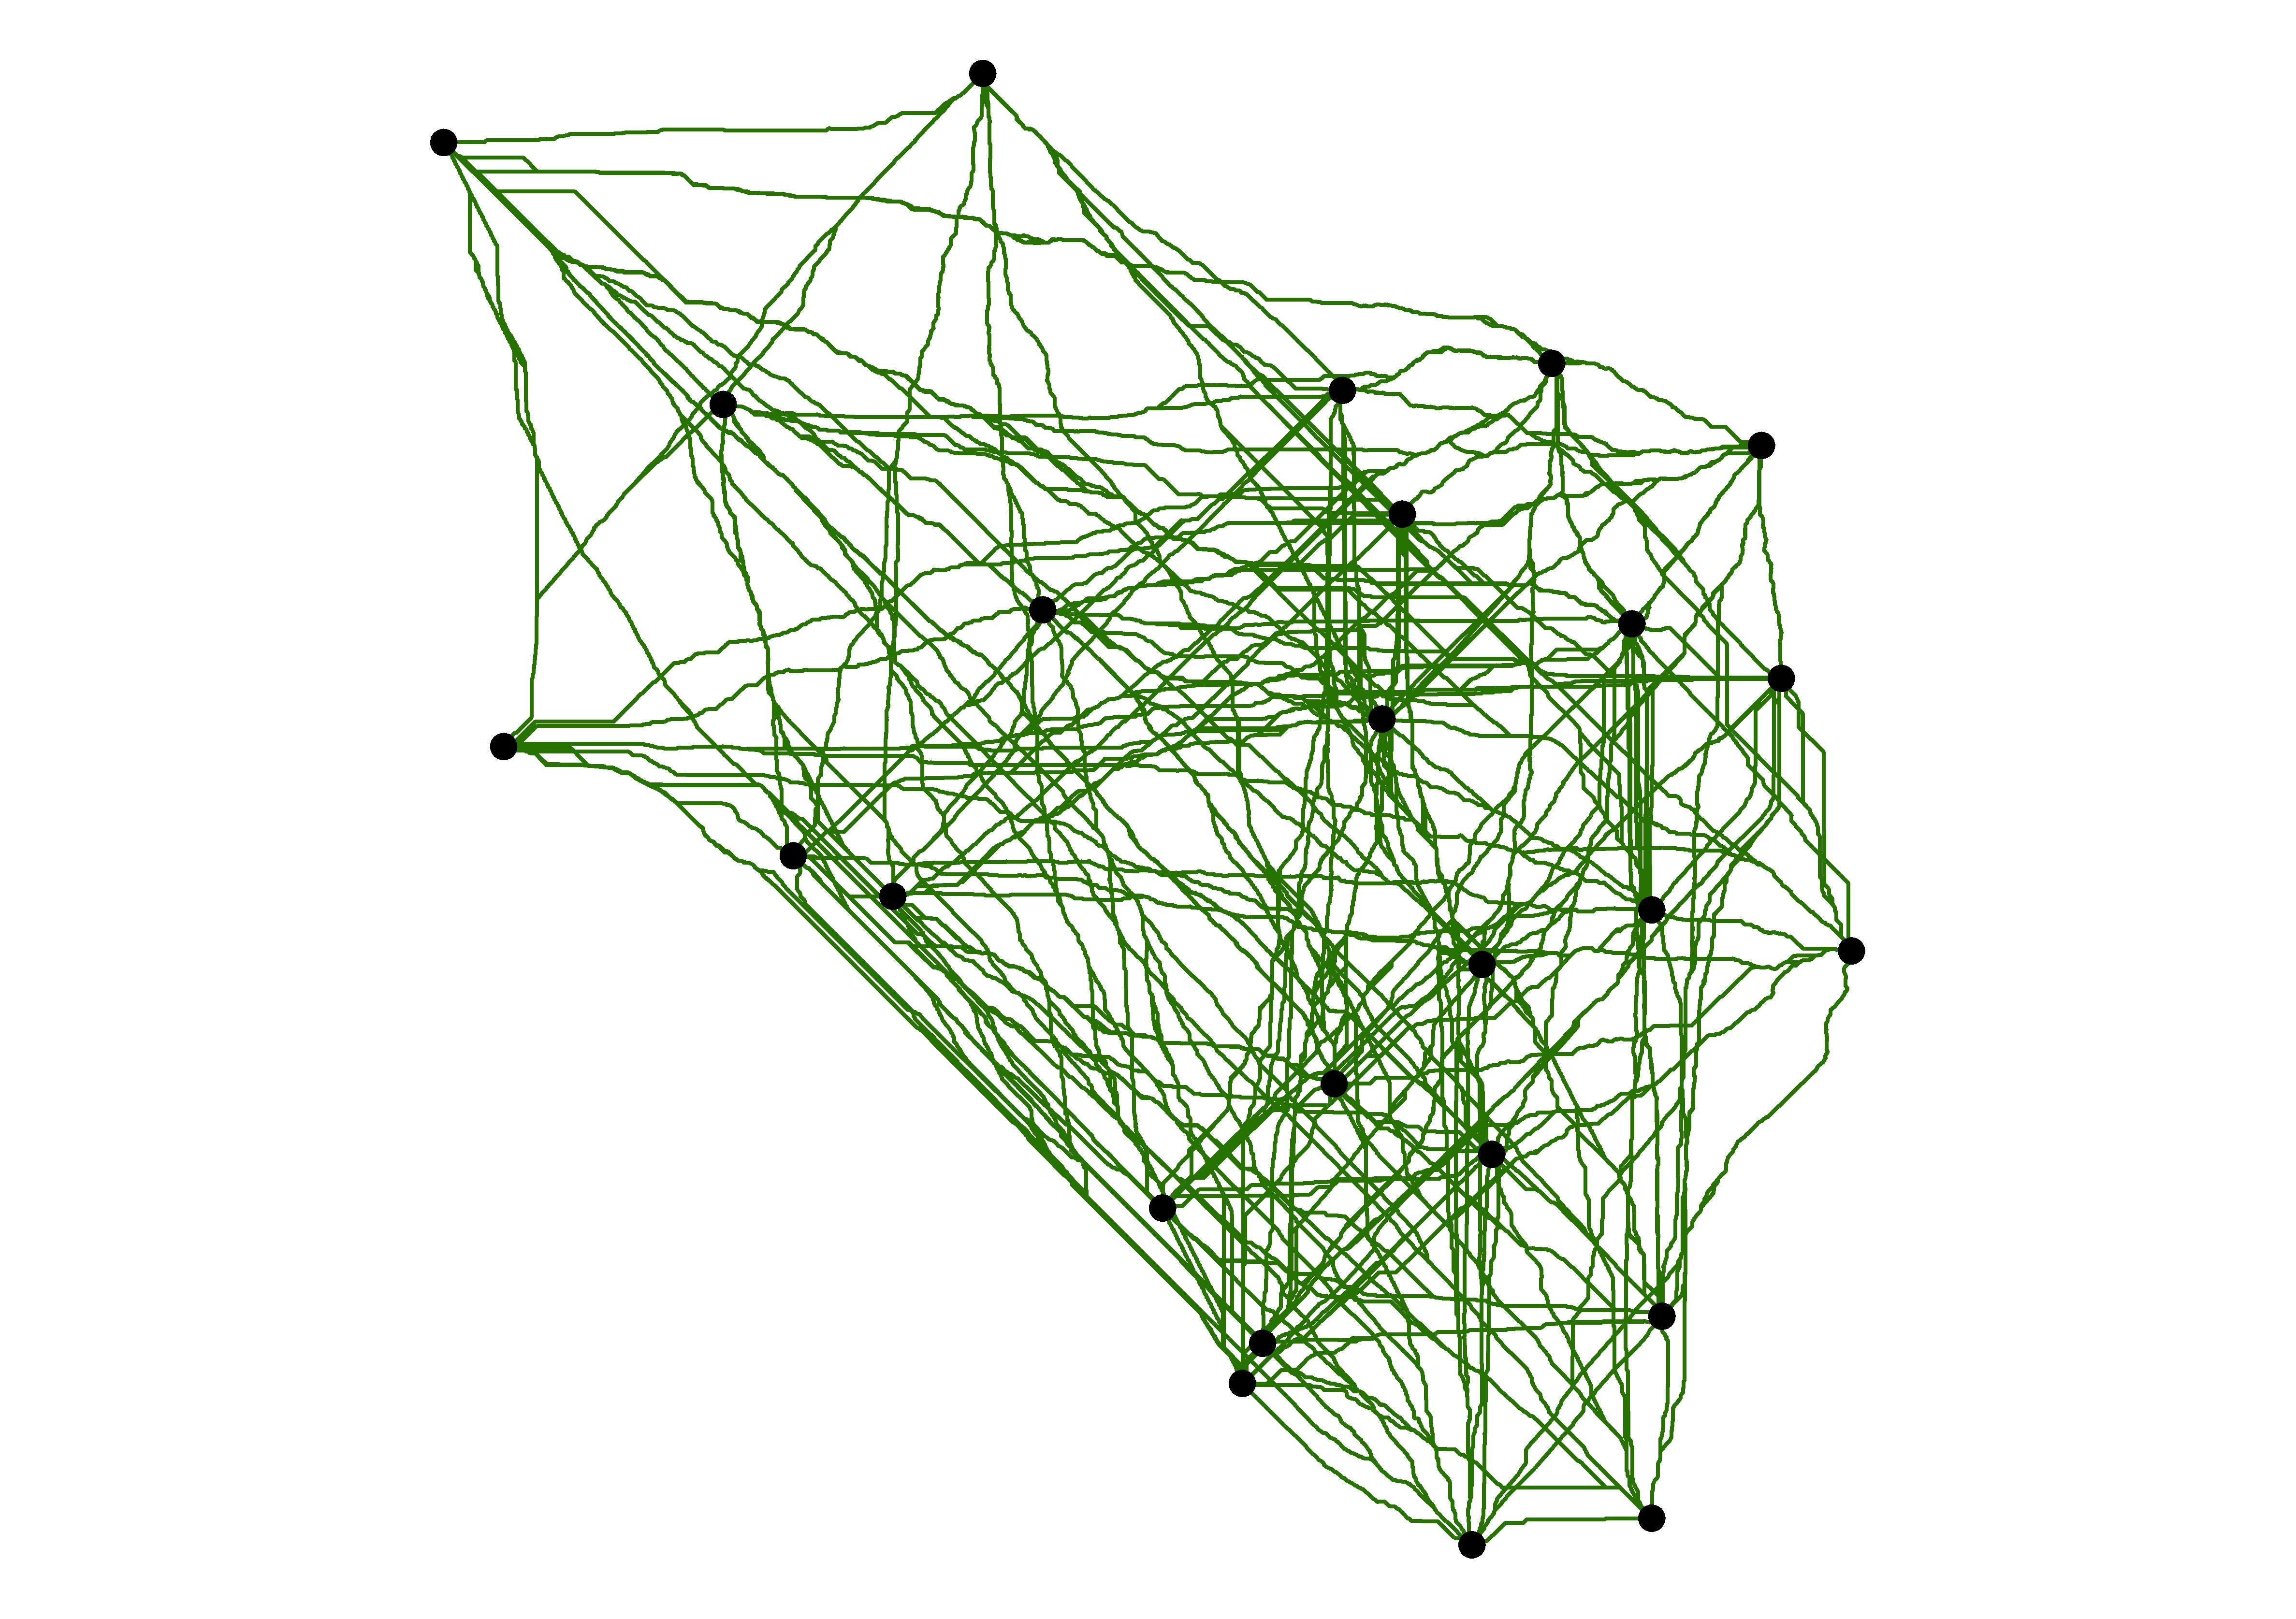
\includegraphics[width=0.7\linewidth]{../LCPs}
\caption{Accumulated least-cost paths between all sites.}
\label{fig:LCPs}
\end{figure}

\section{Simulating Networks Using Spatial Interaction Models}

\subsection{Preliminary Data Modeling}
\paragraph{}
Prior to running the selected models exploratory data analysis will be performed using the proximal point analysis and maximum distance network models. While the limitations of these models are apparent (Section 2.5) they can nevertheless enable a basic understanding of which distances or number of nearest neighbors results in different levels of network connectivity. These simple metrics will help calibrate the more complex models chosen for interaction simulations.

\paragraph{}
Running the proximal point analysis model on the site data using $k$ values of 1, 2, 3, 4, 5, 7, and 9 illustrates how the interaction network becomes more connected as each settlement is forced to connect with an increasing number of nearest neighbors (Figure \ref{fig:PPA}). When $k$ equals 1-2 the connectivity network exists only through shorter distance links. Increasing $k$ up to 3-5 enables settlements to make medium distance journeys and to begin making more unrealistic long distance trips. At $k$ values of 7 and 9 it is apparent that the network is too highly connected to accurately resemble any nuance of reality. It is extremely unlikely that some of the smaller sites would have the means to sustain such expensive interactions. 

\paragraph{}
Similarly, running the maximum-distance network model, using distances of 25km, 50km, 75km, 85km, 100km, 125km, and 150km, generates interactions networks with compounding complexity (Figure \ref{fig:MDN}). At distances of 25km and 50km the study region remains extremely disconnected. Increasing the distance threshold to 75km results in highly connected southern Etruria and a partially fragmented northern Etruria (which is interesting given the general consensus that the south developed more rapidly). It is not until a threshold of 85km that every site is included within the network though there are still large disparities between the northern and southern regions. Finally, values of over 100km begin to yield overly connected networks which result in the smallest of settlements making great journeys. Overall, it seems that a network in which the average node has about 5 edges and a distances threshold of about 100km would be the most representative of a highly connect, though still constrained, spatial interaction system.  


 

\subsection{Radiation Model}
\paragraph{}
To operationalize the radiation model code was developed following \cite{Bar12} with one exception. The term  $T_{i}$, which is supposed to be a proportion of the total population originating at each site, will instead consider the settlement size estimate at a given location. Alternatively, $T_{i}$ could be a ratio of the settlement site size to the total of all sizes. Any value which accurately scales calculations by the estimates at the origins is acceptable. Since $M_{i}$ is also equal to the origin estimate, equation \ref{eq:originalRad} from section 2.3 therefore becomes,
						
				
				\begin{equation}						
				T_{ij} = \frac{(M_{i}^2*N_{j})}{(M_{i}+S_{ij})(M_{i}+N_{j}+S_{ij})}
				\label{eq:newRad}	
				\end{equation}
						
giving $Mi^2$ in the numerator. The radiation model has no parameters so there is no further preparations necessary. The code formats the data into an origin-destination matrix and then  carries out equation \ref{eq:newRad} for each pair of locations resulting in a matrix of relative spatial interaction between them. Since many flows between sites will have near-zero values the network is filtered by removing all edges with a weight that is less than one percent of the largest edge weight value. 

\subsection{Ariadne Model}
	
\paragraph{}
Before any interaction data can be harvested from the Ariadne model it must be configured for our study area. We must prescribe a distance which represents the average trip length one could complete in a day and therefore in a single journey. Based on conclusions aggregated by \cite{BevForthcoming} the average travel speed over a full day for a pedestrian ranges from 2.5km/h to 5km/h depending on the load they may be carrying. In contrast, horses would have reached speeds of 4km/h - 8km/h when carrying packs and 10km/h - 30km/h when utilized solely for riding. If we take a full day's travel to be about 12 hours then the maximum distance traveled by a pedestrian in a day is approximately 60km. For travel on horseback (taking the upper limit of the speed of a pack horse) it would be possible to travel about 96km. In reality, a riding horse could reach much higher speeds and therefore cover distances well over 100km. It is apparent that there is a division in the limitations of these two different travel modes and so both will be considered in this model. In each scenario anything longer than these values will incur large costs so that these trips will only be chosen if there are ample benefits to outweigh the costs. An additional distance must be specified in the model which denotes the point at which very close settlements are considered as one entity (``coarse-graining''). A value of 5km is sufficient for this measure, which would combine settlements where pedestrians could interact with travel times around 1-2 hours regardless of mode, though the site distribution for this study is unaffected since all settlements are separated by values larger than the this threshold. 

\paragraph{}
Finally, the model must be parameterized. Ariadne's four parameters $k$, $\lambda$, $j$, and $\mu$ must be tweaked in order to find a network which conforms to a theoretical scenario. Drawing on the experience of previous research \citep{KnaRivEva11} we will initiate parameterization using values of $k$ = 1.0, $\lambda$ = 4.0, $j$ = -2.0, and $\mu$ = 0.1. For our purpose, we search for a network which allows many nodes to interact, while ensuring the network does not become overly connected. For instance, we should not see small settlements that are sustaining many long distance journeys and no settlements should be should be sustaining strong long distance links since it would have been prohibitively expensive. In effect, we are seeking a network which represents two different scales (short vs. long) which are differentiated by their strength (strong vs. weak). Parameterization is a relative process which requires exploration. While it is arguably unsound to prescribe parameters to find a satisfying network we can nevertheless defend our choice by comparing it to other less appealing parameter options given that all other model values are held constant. Sensitivity of parameters was therefore tested by running the model and, in turn, either doubling or halving each initial parameter while holding all others constant (Figure \ref{fig:60kmAll} and Figure \ref{fig:100kmAll}) and assessing changes to the resulting networks.

\begin{figure}
\centering
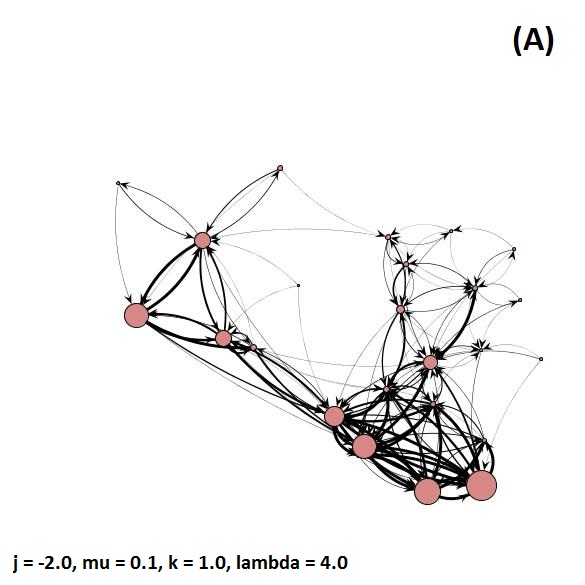
\includegraphics[width=0.35\linewidth]{../ExploratoryModelAnalysis/Ariadne/60/1lcptest_j-02_00-m00_100-k001_00-l004_00}
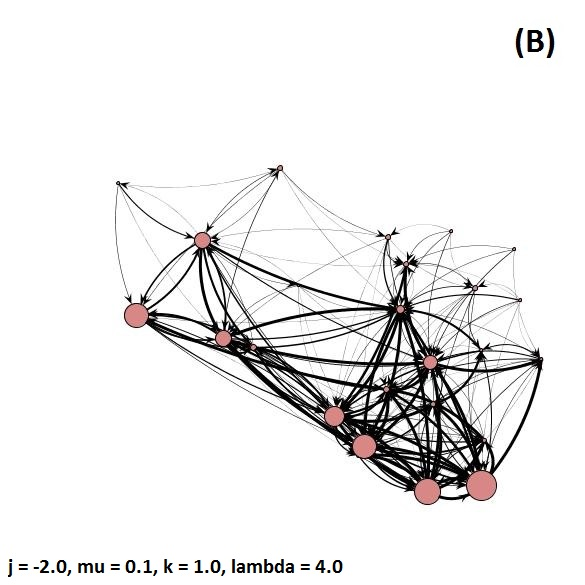
\includegraphics[width=0.35\linewidth]{../ExploratoryModelAnalysis/Ariadne/100/1lcptest_j-02_00-m00_100-k001_00-l004_00}
\caption{Ariadne model runs with initial parameters for average journeys of 60km and 100km}
\label{fig:initParams}
\end{figure}

\paragraph{}
By visually examining each network from the parameter tests it is possible to distinguish which values will provide the best representation of interaction. For the system assuming 60km average trip lengths it appears that increasing $k$, decreasing $\lambda$, or decreasing $\mu$ will cause the network to become slightly under-connected while decreasing $k$ or increasing $\lambda$ will result in slightly over-connected networks. Other parameter changes resulted in minimal deviations and overall the system is insensitive. As a result, the initial parameters will be used to produce networks with ideal conditions (Figure \ref{fig:initParams} A) at this scale. It is evident that employing the same initial values for a model accommodating longer trips (Figure \ref{fig:initParams} B) the network will be too dense and permit too many strong long distance relationships. Doubling $k$ or halving $\lambda$ give more accurate representations and therefore by increasing $k$ from 1 to 1.5 and decreasing $\lambda$ from 4 to 3 it is possible to take a balanced approach to settling on parameters to produce a preferable interaction system.

\paragraph{}
Due to the stochastic nature of Ariadne it is necessary to an average of many model runs. This ensures that fluctuations which may account between different model runs are accounted for within the analysis of this research. 
All networks produced from this model were filtered to remove near-zero edges using a cutoff value produced by dividing the average edge weight by seven times its standard deviation. This method was chosen due to the fact that the distribution of network edges was always similar but that the maximum edge weight value could vary enough do that filtering using a cutoff based upon it would create very different networks.  


\subsection{Agent-based Model}


\paragraph{}
To take an agent-based approach to simulating spatial interaction for this study region some changes were imposed upon the TravellerSim model introduced earlier (section 2.5). First, the local vision was increased from 25km to match the journey limitations proposed for use in the Ariadne model (60km and 100km). This change reflects the additions of horse related transportation and a general increase in spatial awareness that would have been assumed to accompany intensified relationships with the landscape and larger settlements. For this research only the longer distance constraint could be utilized due to the fact that the shirt distance constraint resulted in an extremely fragmented network (figure \ref{fig:agent60}). Next, the attractiveness of each settlement was calculated each round rather than randomly selecting three from those within a human agent's vision. The original authors \citep{GraSte08} explain that this limitation acted primarily as a computation shortcut to prevent lengthy simulation run times and they rationalize this decision by adding that it would have reflected an agent's limited knowledge of their surroundings. It is unknown whether the authors realized that this limitation was the basis for which their model became stochastic (every run yields slightly different results); however, this shortcut was removed due to advances in computing capabilities and that the larger, more urbanized sites would have likely had an increased knowledge of the region. As a result, the model has become deterministic. To test the stability of the interaction system resulting from this model slight deviations to a site's importance were administered at end of each iteration within the simulation. Each site's importance was increased or decreased with equal probability by a value which was randomly generated according to the Poisson distribution using its current importance as the lambda parameter. Overall, model runs using this alteration (Figure \ref{fig:agentFluctuations}) manifested remarkably similar structure highlighting the stability of process being modeled. Another effect of this approach is that the model results will be interpreted statistically, similarly to the Ariadne networks, using the average many networks.  

\begin{figure}
\centering
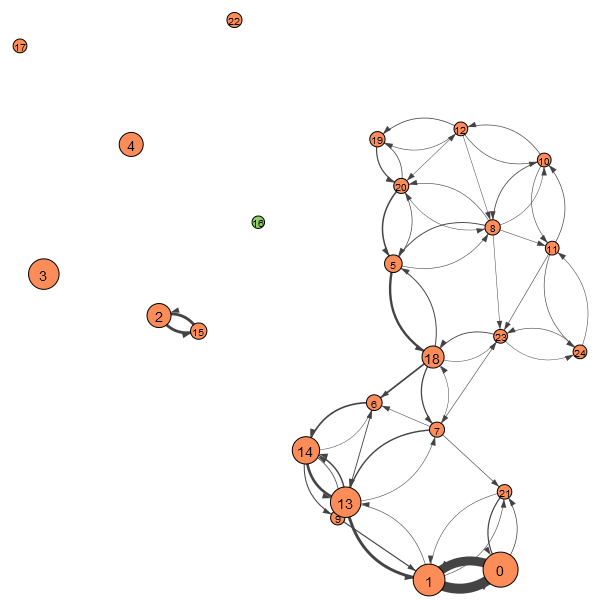
\includegraphics[width=0.35\linewidth]{../BeforeViz/agent60}
\caption{Disconnected network from agent-based framework (60km).}
\label{fig:agent60}
\end{figure}


\paragraph{}
Parameterization of the agent model includes choosing the logistical variables of how many human agents should start at each settlement agent and how many iterations the model should be run for, as well as model variables consisting of values for the difficulty of communication and benefits from resources. Testing the simulations with varying numbers of agents or iterations holding other parameters constant demonstrated that the model was insensitive to these logistical inputs. Five agents and 10 iterations were chosen to ensure enough complexity in the model without utilizing unnecessary computing time. The model variables were tested in a similar manner; values for the range .01 to 5 were tested for each parameter holding the other one constant. Again, the system structure proved extremely resilient to these deviations so values of 1 were employed for both variables. Networks produced from the agent-based model do not results in near-zero values for edge weights and therefore do not need to be filtered.   

\section{Network Analysis Metrics}

\subsection{Node-level Metrics}

\paragraph{}
Questions pertaining to the context of individual  sites can only be achieved using metrics which consider the properties for each node within a network. Equally vital is the ability to validate the accuracy of each network by comparing the properties developed at each settlement to observed data and therefore the overall usefulness it contributes to archaeological studies. Further, Changes within these attributes will allow the interpretations that will ultimately help answers specific questions regarding Poggio Civitate's purpose in the region and the effects of its destruction. This section will establish and review which node-level metrics will be employed for site-specific analysis.


\subsubsection{Interaction Strength}
\paragraph{}
Interaction is an output of each of the models which does not require any additional computing. Using visualization it is possible to quickly notice where interactions are predicted to have occurred more strongly. It is also possible to take the sum of either all incoming or outgoing interaction for each node. This translates roughly into how much trade, information, or people may have been transferred to this site in comparison to all other sites within the region. 

\subsubsection{Degree Centrality}
\paragraph{}
The degree is the number of edges connected to a node. Since this research looks at directed networks we must differentiate between the number of edges arriving at a node and the number of edges originating at a node or, more simply, the ``in degree'' and ``out degree''. A settlement is considered more important if it has a higher degree and therefore has many other settlements connecting to it \cite[64]{RodComSla06}.  





\subsubsection{PageRank}
\paragraph{title}
Originally developed by Google as a mechanism to ranks web sites, the PageRank algorithm is useful in many networks for ranking nodes based on the structure of incoming links \citetext{\citealp{PageRank}; \citealp{LanMey04}}. It was first suggested for use within archaeological networks by Evans, Knappett, and Rivers \citeyearpar{KnaEvaRiv08} who adopted it due to its ability to account for weighted links and nodes which were characteristic of their simulated interaction networks. Specifically, they were able to find settlements or nodes which ``punched above their weight'' which means they has a high PageRank value given their node size and is likely acting as a gateway community between clusters (8-11). Due to this, it will be particularly useful for measuring the importance of smaller sites such as Poggio Civitate which have been theorized to possibly had much importance.


\subsubsection{HITS (Authorities and Hubs)}
\paragraph{}
The HITS algorithm \citetext{\citealp{Kle99}; \citealp{PageRank}} is similar to PageRank in that it uses links to find nodes of importance but it computes a value for both incoming links (``authorities'') and outgoing links (``hubs''). This metric will provide validation against the PageRank values and will be helpful in distinguishing between ``supply-side'' and ``demand-side'' relationships of nodes.

\subsection{Network-level Metrics}
\paragraph{}
A core component of this study is to evaluate an entire network, which is representative of a region, in order to compare results from differing models and parameters. Newman \citeyearpar{New03} suggests that there are features of networks which arise frequently and are therefore helpful for analysis such as the small-world effect, transitivity/clustering, degree distributions, network resiliency, mixing patterns, and community structure. Methods for measuring each of these properties which is pertinent to this study will be reviewed along with network measures and indices \citep{RodComSla06}, which are typically employed for analysis within transportation studies. Indices compare one attribute against another to express more complex relationships within a network's structure. This section will outline the network level metrics which will be calculated for systems in this research in order to understand their structures as well as facilitate comparison.


\subsubsection{Average Node Degree}
\paragraph{}
Average node degree is similar to the degree measure described previously in the nodes-level metrics except that it does not distinguish between incoming and outgoing relationships. It is, in effect, an average for all degree values calculated for individual nodes. Higher degrees are associated with more connected networks.  

\subsubsection{Assortativity Coefficient (Degree and Size)}
\paragraph{}
Assortativity measures the similarity of connections in the graph with respect to a given attribute. In this case, the relationship between connectivity and total interaction flowing through a node is being calculated. A higher coefficient means there is a stronger relationship between these two variables within the network \citeyearpar{New03a}. 

\subsubsection{Diameter}
\paragraph{}
The diameter is a measure of the shortest path (number of links traversed) between the most distanced nodes in a network. It is a helpful measure because more connected networks will tend to have smaller diameters and it can be useful to measure how the diameter changes as the network is altered in order to get an idea of changing connectivity. 


\subsubsection{Transitivity/Average Clustering}
\paragraph{}
A clustering coefficient , which measures transitivity, is most easily described in terms of social networks in which it is the mean probability that a friend of a friend is also your friend. In network terminology this relationship is referred to as a triangle and the coefficient measures the ratio of all triangles present in a network compared to the total possible triangles \cite[11-12]{New03}. Similarly, to get a network-level measure of transitivity it is possible to calculate the mean cluster coefficient from individual nodes. The coefficient will provide a global insight into the clustered nature of the produced networks.


\subsubsection{Beta Index}
\paragraph{}
The beta index measure network connectivity through the ratio of the number of links to the number of nodes. Simpler networks with less than 1 cycle and are not very connected have a beta index of 1 while those which are connect and have more than 1 cycle have a beta index greater than 1. Holding the number of nodes constant, the higher the number of links means there are more paths possible which will correspond to a higher beta index. 

\subsubsection{Gamma Index}
\paragraph{}
The Gamma index compares the number of links with the maximum number of possible links. The values range from 0 to 1 with higher values representing more connected networks. The Gamma index is especially useful for measuring changes in networks over time. It is unique because it provides a measure of connectivity independently of nodes.



\paragraph{}	
In all of the models, network visualizations offer the first clues into system structures and how Murlo factors within the region. A filter is applied to the agent model and Ariadne due to edges being calculated between all node pairs yet many of them having near-zero values. Following the visualization a table of results for each the node-level metrics and the network-level metrics will be reported. Lastly, Poggio Civitate (node 16) will be removed from the input data and the models will be re-run holding everything else constant and new data will be recorded. 


\chapter{Results}
\paragraph{}
A visualization, network-based metrics, and individual node metrics will be provided for each model for a system including Murlo and then again after removing this node from the study region to mimic its destruction. Graphs will also be presented to illustrate the changes in interaction between the two scenarios within each framework. Interaction deviations will be reported as percent increase/decrease from total interaction (incoming and outgoing) at each node for networks that include all settlements within the study region. Values of $999$ within the following tables represents instances where a metric calculation is not available for a node.


\section{Radiation Model} 

\paragraph{}
Network results of the radiation model indicate that Poggio Civitate was not a highly connected node and, therefore,  that its spatial orientation would not have granted it superior network advantages. Rather, this model indicates that Murlo would have actually been quite isolated generally lacking the ability to achieve outward interaction. Even the sole incoming interaction to Poggio Civitate is evidence against its role as a central node within the network since it is the weakest interaction within the entire system. A low PageRank value confirms that it was not, in fact, punching above its weight and did not have a large importance in the overall network connectivity. 

\paragraph{}
A Medium transitivity value suggests that there is some mild neighborhood associations within the network but that it is not the defining factor. Frequent weak long-distance interactions in the visualization confirm that small communities do not prevail as the core structure. Interestingly, upon the removal of Murlo, there is slight increase in the overall connectivity of the network. It is expected that beta index will increase with the removal of any nodes (links/nodes), especially minimally connected ones, but values for the transitivity and gamma index also support this slight trend. The gamma index is especially indicative here since it independent of the number of nodes. Globally, the structure seems not to be influenced and is corroborated by the fact that the network diameter remains unchanged. The new system state supports approximately five percent increases in interaction for nodes 4 and 5 while node 22 approaches a 20 percent gain in interaction. 
\subsubsection{Before}

\begin{figure}[H]
\centering
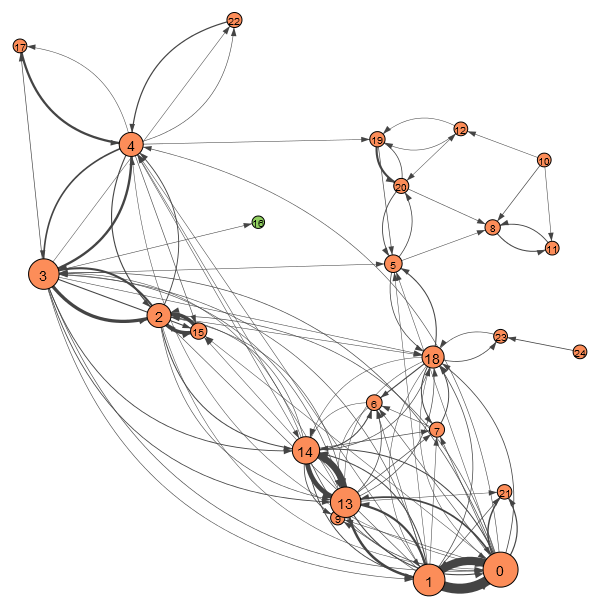
\includegraphics[width=0.35\linewidth]{./BeforeViz/radModel}
\caption{Visualization of a single radiation model run including Murlo.}
\label{fig:radModelBefore}
\end{figure}

\begin{figure}[H]
\centering
\tiny
\begin{tabular}{|c|c|c|c|c|c|c|}
\hline Metric & Assortativity & Diameter & Average Degree & Transitivity & Beta & Gamma \\ 
\hline Radiation Model (Before) & -0.06080357 & 5 & 8.72 & 0.44292804 & 4.36 & 0.1744 \\ 
\hline 
\end{tabular} 
\end{figure}

\begin{figure}[H]
\centering
\tiny
\begin{tabular}{|c|c|c|c|c|c|c|c|}
\hline	Node	&	Interaction In	&	Interaction Out	&	Degree In	&	Degree Out	&	PageRank	&	Hubs	&	Authorities	\\
\hline	0	&	108.75090365	&	111.16414012	&	8	&	13	&	0.06751344	&	0.14177813	&	0.40598155	\\
\hline	1	&	96.07389215	&	122.16387527	&	5	&	12 &	0.06478559	&	0.44423172	&	0.13413920	\\
\hline	2	&	67.87638768	&	56.74109960	&	7	&	7	&	0.06741936	&	0.02266724	&	0.02894542	\\
\hline	3	&	33.31327788	&	68.03210348	&	6	&	12	&	0.03977904	&	0.03765628	&	0.02027152	\\
\hline	4	&	49.93975449	&	25.07446728	&	7	&	8	&	0.03640718	&	0.01098481	&	0.01785142	\\
\hline	5	&	15.57227832	&	7.52633653	&	6	&	3	&	0.03935866	&	0.00092203	&	0.00707285	\\
\hline	6	&	19.07883554	&	2.10864198	&	6	&	2	&	0.03306262	&	0.00306255	&	0.01858651	\\
\hline	7	&	13.05993630	&	6.04581589	&	5	&	2	&	0.02289676	&	0.00165243	&	0.01460570	\\
\hline	8	&	9.06115422	&	5.47008547	&	4	&	1	&	0.09012996	&	0.00000000	&	0.00001391	\\
\hline	9	&	27.85788453	&	22.08000000	&	4	&	2	&	0.02778622	&	0.03360924	&	0.04525178	\\
\hline	10	&	0.00000000	&	4.73429952	&	0	&	3	&	0.00623404	&	0.00000042	&	0.00000000	\\
\hline	11	&	6.67781494	&	4.44444444	&	2	&	1	&	0.08419627	&	0.00000072	&	0.00000001	\\
\hline	12	&	2.59301085	&	1.79757322	&	2	&	2	&	0.00909824	&	0.00000210	&	0.00000296	\\
\hline	13	&	94.33529348	&	113.27241140	&	8	&	11	&	0.10268830	&	0.14690874	&	0.13064157	\\
\hline	14	&	78.80731418	&	62.97010450	&	9	&	10	&	0.07948022	&	0.08401978	&	0.11709181	\\
\hline	15	&	38.35885414	&	28.57142857	&	5	&	1	&	0.04194336	&	0.00969919	&	0.01136807	\\
\hline	16	&	1.30662021	&	0.00000000	&	1	&	0	&	0.00688343	&	0.00000000	&	0.00050247	\\
\hline	17	&	3.35917313	&	16.66666667	&	2	&	1	&	0.00866548	&	0.00348936	&	0.00101027	\\
\hline	18	&	23.34730839	&	24.57352717	&	9	&	8	&	0.06042608	&	0.01249645	&	0.02455853	\\
\hline	19	&	5.22510994	&	19.24215940	&	3	&	3	&	0.02471582	&	0.00020864	&	0.00013203	\\
\hline	20	&	19.71195355	&	8.70209059	&	3	&	3	&	0.04181020	&	0.00035005	&	0.00006471	\\
\hline	21	&	9.95700623	&	9.26644932	&	3	&	1	&	0.01146410	&	0.04412081	&	0.02097623	\\
\hline	22	&	2.45524664	&	7.26744186	&	2	&	1	&	0.00862441	&	0.00152152	&	0.00051184	\\
\hline	23	&	6.61742424	&	2.08793908	&	2	&	1	&	0.01839718	&	0.00060137	&	0.00041967	\\
\hline	24	&	0.00000000	&	3.33333333	&	0	&	1	&	0.00623404	&	0.00001641	&	0.00000000	\\
\hline 
\end{tabular} 
\end{figure}

\subsubsection{After}

\begin{figure}[H]
\centering
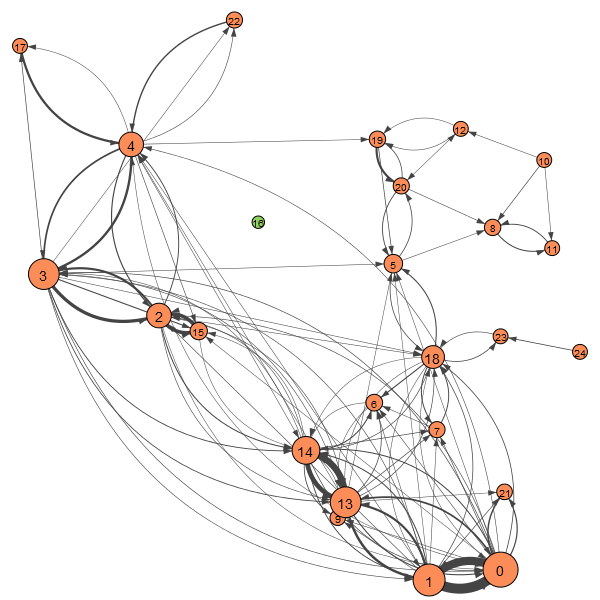
\includegraphics[width=0.35\linewidth]{./AfterViz/radModel}
\caption{Visualization of a single radiation model run excluding Murlo.}
\label{fig:radModelAfter}
\end{figure}

\begin{figure}[H]
\centering
\tiny
\begin{tabular}{|c|c|c|c|c|c|c|}
\hline Metric & Assortativity & Diameter & Average Degree & Transitivity & Beta & Gamma \\ 
\hline Radiation Model (After) & -0.06149662 & 5 & 8.8 & 0.46039604 & 4.58333333 & 0.19097222 \\ 
\hline 
\end{tabular} 
\end{figure}

\begin{figure}[H]
\centering
\tiny
\begin{tabular}{|c|c|c|c|c|c|c|c|}
\hline	Node	&	Interaction In	&	Interaction Out	&	Degree In	&	Degree Out	&	PageRank	&	Hubs	&	Authorities	\\
\hline	0	&	108.87945837	&	111.28995232	&	8	&	13	&	0.06801471	&	0.14163172	&	0.40324103	\\
\hline	1	&	96.24280876	&	122.25482314	&	5	&	12	&	0.06532898	&	0.44076822	&	0.13419461	\\
\hline	2	&	68.33916527	&	58.24965169	&	7	&	7	&	0.06611103	&	0.02357307	&	0.02983908	\\
\hline	3	&	35.08523104	&	67.13766184	&	6	&	11	&	0.04047912	&	0.03834858	&	0.02094712	\\
\hline	4	&	51.88176247	&	26.33777091	&	7	&	8	&	0.03687712	&	0.01148110	&	0.01822987	\\
\hline	5	&	16.86599343	&	7.52633653	&	7	&	3	&	0.04070164	&	0.00092053	&	0.00847579	\\
\hline	6	&	19.07883554	&	2.10864198	&	6	&	2	&	0.03333116	&	0.00305249	&	0.01855696	\\
\hline	7	&	13.05993630	&	6.04581589	&	5	&	2	&	0.02306993	&	0.00164857	&	0.01457395	\\
\hline	8	&	9.06115422	&	5.47008547	&	4	&	1	&	0.09093085	&	0.00000000	&	0.00001483	\\
\hline	9	&	27.85788453	&	22.08000000	&	4	&	2	&	0.02786109	&	0.03345954	&	0.04514594	\\
\hline	10	&	0.00000000	&	4.73429952	&	0	&	3	&	0.00625000	&	0.00000046	&	0.00000000	\\
\hline	11	&	6.67781494	&	4.44444444	&	2	&	1	&	0.08489646	&	0.00000077	&	0.00000001	\\
\hline	12	&	2.59301085	&	1.79757322	&	2	&	2	&	0.00909570	&	0.00000236	&	0.00000405	\\
\hline	13	&	94.47431256	&	114.20909230	&	8	&	12	&	0.10355927	&	0.14659166	&	0.13024651	\\
\hline	14	&	80.00784943	&	63.28116180	&	10	&	10	&	0.08076402	&	0.08412710	&	0.11706552	\\
\hline	15	&	38.48556453	&	29.43232320	&	5	&	2	&	0.04082815	&	0.01116279	&	0.01174679	\\
\hline	16	&	0.00000000	&	0.00000000	&	999	&	999	&	999	&	999	&	999	\\
\hline	17	&	3.51731602	&	16.66666667	&	2	&	1	&	0.00878597	&	0.00355765	&	0.00108121	\\
\hline	18	&	23.44998253	&	24.63662226	&	9	&	8	&	0.06125753	&	0.01268673	&	0.02454451	\\
\hline	19	&	5.26560692	&	19.60770605	&	3	&	3	&	0.02481946	&	0.00028580	&	0.00014456	\\
\hline	20	&	19.71195355	&	8.70209059	&	3	&	3	&	0.04209021	&	0.00041828	&	0.00007691	\\
\hline	21	&	9.95700623	&	9.26644932	&	3	&	1	&	0.01151002	&	0.04375314	&	0.02090135	\\
\hline	22	&	2.55094330	&	8.96057348	&	2	&	1	&	0.00868424	&	0.00191272	&	0.00054308	\\
\hline	23	&	6.61742424	&	2.08793908	&	2	&	1	&	0.01850335	&	0.00060007	&	0.00042632	\\
\hline	24	&	0.00000000	&	3.33333333	&	0	&	1	&	0.00625000	&	0.00001664	&	0.00000000	\\
\hline 
\end{tabular} 
\end{figure}

\subsubsection{Interaction Shifts}

\begin{figure}[H]
\centering
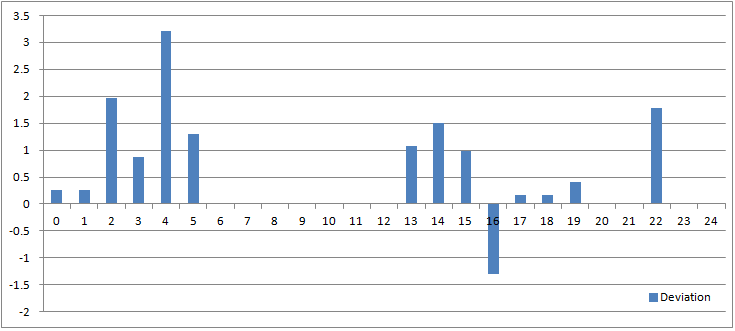
\includegraphics[width=0.7\linewidth]{../NodeDeviations/Radiation}
\caption{Total interaction shift by node for radiation model.}
\label{fig:RadiationShift}
\end{figure}

\begin{figure}[H]
\centering
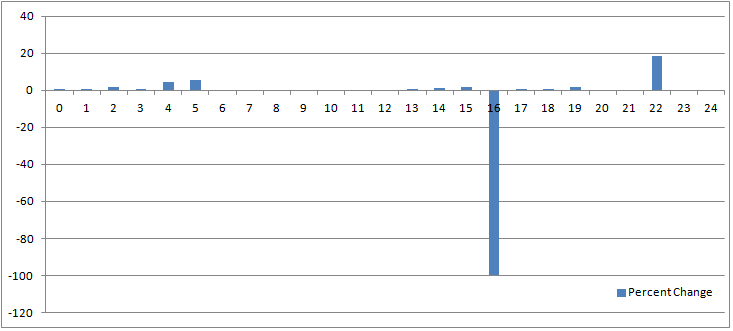
\includegraphics[width=0.7\linewidth]{../NodeDeviations/RadiationPercent}
\caption{Percent total interaction by node for radiation model.}
\label{fig:RadiationPercent}
\end{figure}


\section{Ariadne Model}

\paragraph{}
In each scenario, the network-level metrics converged to steady values within 25 averaged model runs (Figure \ref{fig:ConvergeAriadneB60}, \ref{fig:ConvergeAriadneB100}, \ref{fig:ConvergeAriadneA60}, \ref{fig:ConvergeAriadneA100}). At the lower distance threshold the Ariadne model indicates that on average Poggio Civitate would have sustained 2-3 outgoing interactions and 0-1 incoming interactions though they would have been among some of the weakest links within the network. Increasing the distance threshold does not have an impact on Murlo's connectivity despite the fact the overall increase in connectivity suggested by a decreasing diameter value. Both model variations produce PageRank and HITS values that are extremely small and therefore confirm Poggio Civitate's relative lack of importance within the system.   

\paragraph{}
High transitivity values suggest strong neighborhood effects within all of the Ariadne model results. It is easy to visually extract communities in the lower distance threshold results though the longer distance threshold results present an interesting deviation for settlements in the northeast. The increased travel distance capabilities seem to have decreased the frequency with which these sites interact with themselves. Instead of forming their own community they tend to explicitly interact with larger more distant nodes. It is difficult to quantify changes within the Ariadne networks after the destruction of Murlo. For both variations of the model the metrics present mixed evidence for whether or not the system becomes more connected. Additionally, none of the resulting values represent large deviations so the variations within the measurements is likely due to the stochastic nature of the model. Ultimately, the removal of Poggio Civiate does not cause significant shifts within the network. There is a split in the number of nodes which gain interaction and those which lose interaction for the 60km threshold. Nodes 3, 5, 9, 20 , and 22 show the largest increases with node 5 (Chiusi) having the highest at about 21 percent. In contrast, nodes 6, 14, 15, 23, and 24 decrease the most significantly with maximum loses of 20 percent by node 15. The 100km threshold is dominated by decreasing interaction shifts. Seventeen nodes proved to have decreased interaction with 7 of the nodes (0, 1, 9, 11, 13,and 19) having loses between 20-30 percent. Nodes 4, 8, and 22 show substantial gains of 10-20 percent. 

\subsubsection{Before - 60km}

\begin{figure}[H]
\centering
\includegraphics[width=0.35\linewidth]{./BeforeViz/ariadne60}
\caption{Visualization of a single Ariadne model run including Murlo (60km).}
\label{fig:ariadneB60}
\end{figure}

\begin{figure}[H]
\centering
\tiny
\begin{tabular}{|c|c|c|c|c|c|c|}
\hline Metric & Assortativity & Diameter & Average Degree & Transitivity & Beta & Gamma \\ 
\hline Ariadne (Before: 60km) & -0.05119454	& 4.1600 & 11.6288 & 0.70893446 & 5.8144 & 0.232576\\ 
\hline 
\end{tabular} 
\end{figure}


\begin{figure}[H]
\centering
\tiny
\begin{tabular}{|c|c|c|c|c|c|c|c|}
\hline	Node	&	Interaction In	&	Interaction Out	&	Degree In	&	Degree Out	&	PageRank	&	Hubs	&	Authorities	\\
\hline	0	&	5.15605044	&	10.37701864	&	9.0000	&	7.9600	&	0.06366162	&	0.20301292	&	0.08377937	\\
\hline	1	&	4.78002280	&	10.50274632	&	8.6800	&	8.0400	&	0.06119557	&	0.17104314	&	0.08207493	\\
\hline	2	&	4.37817908	&	4.00114796	&	6.8800	&	7.0400	&	0.05291583	&	0.03862894	&	0.03790744	\\
\hline	3	&	2.33393132	&	4.43702164	&	4.7200	&	5.3600	&	0.03687551	&	0.02893478	&	0.00651458	\\
\hline	4	&	2.45377924	&	2.54004316	&	5.2000	&	6.2400	&	0.03412294	&	0.00863165	&	0.00737997	\\
\hline	5	&	1.40997460	&	1.56258092	&	7.0800	&	6.8800	&	0.04080041	&	0.01457215	&	0.00298033	\\
\hline	6	&	5.68686764	&	2.35101684	&	10.3600	&	7.2000	&	0.06827045	&	0.02891943	&	0.08440798	\\
\hline	7	&	5.83026388	&	2.09756240	&	9.6000	&	7.2000	&	0.06808746	&	0.02972334	&	0.08683485	\\
\hline	8	&	0.89294904	&	0.82821912	&	5.8800	&	5.2400	&	0.02871467	&	0.00346677	&	0.00064527	\\
\hline	9	&	4.70216060	&	2.03496144	&	5.8000	&	6.5600	&	0.04789472	&	0.02954883	&	0.10339356	\\
\hline	10	&	0.04208724	&	0.32914720	&	0.6800	&	4.0000	&	0.00705151	&	0.00033416	&	0.00000596	\\
\hline	11	&	0.16607516	&	0.38591676	&	1.7600	&	3.6800	&	0.01023432	&	0.00225924	&	0.00003969	\\
\hline	12	&	0.20469996	&	0.37850296	&	2.5200	&	4.0000	&	0.01064349	&	0.00004972	&	0.00002770	\\
\hline	13	&	7.94302340	&	10.75129336	&	13.2000	&	8.9200	&	0.09234654	&	0.19751654	&	0.13496315	\\
\hline	14	&	7.99095508	&	7.94175732	&	12.9200	&	9.2400	&	0.09671460	&	0.14070298	&	0.13147314	\\
\hline	15	&	3.65079068	&	1.81954172	&	5.0000	&	6.1600	&	0.04215937	&	0.01908715	&	0.03044919	\\
\hline	16	&	0.02997972	&	0.16392172	&	0.4800	&	2.4000	&	0.00637868	&	0.00080004	&	0.00013414	\\
\hline	17	&	0.20060956	&	0.38098608	&	1.0000	&	2.5200	&	0.00830969	&	0.00058663	&	0.00023103	\\
\hline	18	&	6.67819704	&	3.98009484	&	15.8800	&	8.2800	&	0.09394147	&	0.04162679	&	0.10691481	\\
\hline	19	&	0.44540620	&	0.68159284	&	3.3200	&	4.6000	&	0.01687598	&	0.00126330	&	0.00019425	\\
\hline	20	&	0.89644132	&	0.79641936	&	4.8000	&	4.8000	&	0.02820003	&	0.00252656	&	0.00084704	\\
\hline	21	&	4.74922272	&	1.84394700	&	5.6000	&	6.3600	&	0.04352903	&	0.02428703	&	0.09637430	\\
\hline	22	&	0.18489916	&	0.50844160	&	1.0000	&	3.4400	&	0.00801272	&	0.00059727	&	0.00016563	\\
\hline	23	&	0.86265308	&	0.63189508	&	3.8400	&	5.2000	&	0.02632835	&	0.00780512	&	0.00223517	\\
\hline	24	&	0.01772372	&	0.36116640	&	0.1600	&	4.0400	&	0.00673504	&	0.00407552	&	0.00002649	\\
\hline 
\end{tabular} 
\end{figure}



\subsubsection{Before - 100km}

\begin{figure}[H]
\centering
\includegraphics[width=0.35\linewidth]{./BeforeViz/ariadne100}
\caption{Visualization of a single Ariadne model run including Murlo (100km).}
\label{fig:ariadneB100}
\end{figure}

\begin{figure}[H]
\centering
\tiny
\begin{tabular}{|c|c|c|c|c|c|c|}
\hline Metric & Assortativity & Diameter & Average Degree & Transitivity & Beta & Gamma \\ 
\hline Ariadne (Before: 100km) & -0.05581519 & 3.12 & 11.6576	& 0.69901818 & 5.8288 & 0.233152 \\
\hline 
\end{tabular} 
\end{figure}

\begin{figure}[H]
\centering
\tiny
\begin{tabular}{|c|c|c|c|c|c|c|c|}
\hline	Node	&	Interaction In	&	Interaction Out	&	Degree In	&	Degree Out	&	PageRank	&	Hubs	&	Authorities	\\
\hline	0	&	4.89983452	&	8.32066644	&	12.0000	&	8.2000	&	0.08609509	&	0.19495887	&	0.10330187	\\
\hline	1	&	5.65126364	&	8.52547084	&	12.3200	&	8.2000	&	0.08667110	&	0.20906030	&	0.09710958	\\
\hline	2	&	3.62511764	&	3.19648376	&	10.2400	&	8.0000	&	0.05521474	&	0.03331761	&	0.07971386	\\
\hline	3	&	1.93787876	&	3.88205340	&	5.7200	&	6.6400	&	0.03461827	&	0.06809476	&	0.00905391	\\
\hline	4	&	2.01789728	&	2.54596744	&	6.0400	&	7.4800	&	0.03514888	&	0.01994091	&	0.01186065	\\
\hline	5	&	1.89805124	&	1.26250424	&	9.5200	&	6.5200	&	0.04565378	&	0.01767523	&	0.02984303	\\
\hline	6	&	3.00178612	&	1.37872700	&	7.9600	&	6.1600	&	0.05573647	&	0.01598653	&	0.04757637	\\
\hline	7	&	3.31958660	&	1.40210708	&	7.4400	&	6.7200	&	0.05190872	&	0.02035527	&	0.06626117	\\
\hline	8	&	0.23871468	&	0.57470524	&	2.0000	&	4.6800	&	0.01353769	&	0.00719601	&	0.00115689	\\
\hline	9	&	3.67211716	&	1.25457724	&	5.0800	&	5.8000	&	0.05740215	&	0.02130661	&	0.13629920	\\
\hline	10	&	0.00000000	&	0.23889756	&	0.0000	&	3.4800	&	0.00600000	&	0.00253050	&	0.00000000	\\
\hline	11	&	0.01417564	&	0.30614564	&	0.1200	&	3.8400	&	0.00651435	&	0.00446946	&	0.00000928	\\
\hline	12	&	0.00624680	&	0.24945936	&	0.0400	&	3.4800	&	0.00611249	&	0.00229586	&	0.00000497	\\
\hline	13	&	7.01137616	&	7.85547568	&	16.2800	&	9.7200	&	0.10442409	&	0.15895122	&	0.13394608	\\
\hline	14	&	5.87803916	&	5.48273092	&	16.4400	&	8.7200	&	0.09823489	&	0.11429405	&	0.08765036	\\
\hline	15	&	2.10607784	&	1.24976596	&	4.3600	&	5.9200	&	0.03282420	&	0.01499822	&	0.02142376	\\
\hline	16	&	0.02693540	&	0.13393868	&	0.2400	&	2.2400	&	0.00651135	&	0.00186924	&	0.00038813	\\
\hline	17	&	0.21029052	&	0.36706780	&	0.9600	&	3.0000	&	0.00855607	&	0.00137643	&	0.00096169	\\
\hline	18	&	5.20334476	&	3.14990504	&	18.7200	&	8.6400	&	0.09951101	&	0.04250434	&	0.08257974	\\
\hline	19	&	0.32510116	&	0.49862944	&	1.4000	&	5.1200	&	0.01390796	&	0.00508193	&	0.00077852	\\
\hline	20	&	0.24431164	&	0.50793272	&	1.7200	&	4.2000	&	0.01420025	&	0.00675260	&	0.00065684	\\
\hline	21	&	2.68562484	&	1.27637096	&	4.5200	&	6.0800	&	0.03734474	&	0.01960192	&	0.08137327	\\
\hline	22	&	0.27613360	&	0.51696952	&	1.2400	&	3.9600	&	0.00994763	&	0.00260495	&	0.00115287	\\
\hline	23	&	0.55702292	&	0.48574020	&	0.8800	&	4.8800	&	0.02056382	&	0.00794017	&	0.00575367	\\
\hline	24	&	0.25766600	&	0.40230192	&	0.4800	&	4.0400	&	0.01336026	&	0.00683703	&	0.00114427	\\
\hline 
\end{tabular} 
\end{figure}



\subsubsection{After - 60km}

\begin{figure}[H]
\centering
\includegraphics[width=0.35\linewidth]{./AfterViz/ariadne60}
\caption{Visualization of a single Ariadne model run excluding Murlo (60km).}
\label{fig:ariadneA60}
\end{figure}

\begin{figure}[H]
\centering
\tiny
\begin{tabular}{|c|c|c|c|c|c|c|}
\hline Metric & Assortativity & Diameter & Average Degree & Transitivity & Beta & Gamma \\ 
\hline Ariadne (After: 60km) & -0.05325428	& 4.24 & 11.3152	& 0.72501267 & 5.89333333 & 0.24555556 \\ 
\hline 
\end{tabular} 
\end{figure}

\begin{figure}[H]
\centering
\tiny
\begin{tabular}{|c|c|c|c|c|c|c|c|}
\hline	Node	&	Interaction In	&	Interaction Out	&	Degree In	&	Degree Out	&	PageRank	&	Hubs	&	Authorities	\\
\hline	0	&	5.16036156	&	10.47627292	&	8.8000	&	8.1200 &	0.06567145	&	0.19987111	&	0.08149631	\\
\hline	1	&	5.23551720	&	11.09284644	&	9.0000	&	8.0000	&	0.06563621	&	0.22235560	&	0.08286413	\\
\hline	2	&	4.09353752	&	4.00969188	&	6.1200	&	6.4400	&	0.04967571	&	0.02580089	&	0.03167777	\\
\hline	3	&	2.89074720	&	4.70419836	&	4.5200	&	5.4400	&	0.04058895	&	0.02506704	&	0.00572947	\\
\hline	4	&	2.78197232	&	2.62088708	&	4.4000	&	5.7600	&	0.03650362	&	0.00796128	&	0.00729260	\\
\hline	5	&	1.96130524	&	1.66822824	&	7.3200	&	6.8000	&	0.05233911	&	0.01776381	&	0.00499504	\\
\hline	6	&	4.68613712	&	2.23687204	&	10.2400	&	8.0400	&	0.05813292	&	0.03338689	&	0.07890425	\\
\hline	7	&	5.93678260	&	2.06810156	&	9.4800	&	7.4800	&	0.06582744	&	0.02921817	&	0.11104847	\\
\hline	8	&	0.89386664	&	0.81513760	&	5.7600	&	5.1600	&	0.03269063	&	0.00363226	&	0.00088401	\\
\hline	9	&	5.63912128	&	2.09009756	&	6.2400	&	7.2400	&	0.05185054	&	0.03139406	&	0.13298361	\\
\hline	10	&	0.05323988	&	0.31759552	&	0.7600	&	3.6000	&	0.00783581	&	0.00029367	&	0.00001598	\\
\hline	11	&	0.17444720	&	0.36762904	&	1.6400	&	3.5200	&	0.01275970	&	0.00213306	&	0.00005358	\\
\hline	12	&	0.21906448	&	0.37656312	&	2.2800	&	3.7200	&	0.01182928	&	0.00014320	&	0.00003602	\\
\hline	13	&	7.58302480	&	10.38153036	&	12.6800	&	9.4000	&	0.08908923	&	0.17368731	&	0.14408559	\\
\hline	14	&	7.05862416	&	7.22942652	&	12.8000	&	8.9600	&	0.08587737	&	0.12400177	&	0.10205289	\\
\hline	15	&	2.77190060	&	1.63238884	&	4.1600	&	5.7200	&	0.03197597	&	0.01657326	&	0.01461682	\\
\hline	16	&	0.00000000	&	0.00000000	&	999.0000	&	999.0000	&	999	&	999	&	999	\\
\hline	17	&	0.18248772	&	0.37659180	&	1.0000	&	2.3600	&	0.00857153	&	0.00049695	&	0.00019297	\\
\hline	18	&	6.36680940	&	3.74639724	&	15.4400	&	7.9200	&	0.09275439	&	0.04109655	&	0.09139855	\\
\hline	19	&	0.46389328	&	0.69044140	&	3.4000	&	4.2800	&	0.01935123	&	0.00093279	&	0.00021101	\\
\hline	20	&	1.02280624	&	0.83296720	&	4.7200	&	4.4800	&	0.03604473	&	0.00268190	&	0.00103421	\\
\hline	21	&	4.97287868	&	1.90607880	&	6.3600	&	7.0800	&	0.04788491	&	0.02784183	&	0.10603521	\\
\hline	22	&	0.25915400	&	0.51584076	&	1.0000	&	3.3600	&	0.00957424	&	0.00069252	&	0.00028271	\\
\hline	23	&	0.71327764	&	0.63059148	&	3.2400	&	4.9600	&	0.02103774	&	0.00866464	&	0.00204226	\\
\hline	24	&	0.01100452	&	0.34558552	&	0.0800	&	3.6000	&	0.00649732	&	0.00430945	&	0.00006656	\\
\hline 
\end{tabular} 
\end{figure}

\subsubsection{After - 100km}

\begin{figure}[H]
\centering
\includegraphics[width=0.35\linewidth]{./AfterViz/ariadne100}
\caption{Visualization of a single Ariadne model run excluding Murlo (100km).}
\label{fig:ariadneA100}
\end{figure}

\begin{figure}[H]
\centering
\tiny
\begin{tabular}{|c|c|c|c|c|c|c|}
\hline Metric & Assortativity & Diameter & Average Degree & Transitivity & Beta & Gamma \\ 
\hline Ariadne (After: 100km) & -0.05695306	& 3.08 & 10.9184 & 0.67954338 & 5.68666667	& 0.23694444
 \\ 
\hline 
\end{tabular} 
\end{figure}

\begin{figure}[H]
\centering
\tiny
\begin{tabular}{|c|c|c|c|c|c|c|c|}
\hline	Node	&	Interaction In	&	Interaction Out	&	Degree In	&	Degree Out	&	PageRank	&	Hubs	&	Authorities	\\
\hline	0	&	3.06643424	&	6.07401580	&	10.2400	&	8.0400	&	0.07545583	&	0.12093972	&	0.05003812	\\
\hline	1	&	3.83291536	&	6.11571240	&	10.8000	&	8.5600	&	0.07693095	&	0.17498175	&	0.09110773	\\
\hline	2	&	3.67581112	&	3.18717124	&	9.8000	&	7.6000	&	0.06189563	&	0.05298723	&	0.09799815	\\
\hline	3	&	2.00754312	&	3.94399972	&	5.4800	&	6.5200	&	0.04231811	&	0.10390300	&	0.02089409	\\
\hline	4	&	2.32559364	&	2.70775716	&	6.0400	&	7.2400	&	0.04216085	&	0.03195118	&	0.04732999	\\
\hline	5	&	1.80055964	&	1.22150472	&	9.0000	&	5.8000	&	0.04532250	&	0.02270255	&	0.02714574	\\
\hline	6	&	3.01853756	&	1.26870548	&	7.9200	&	6.2400	&	0.05922607	&	0.02041338	&	0.06835380	\\
\hline	7	&	2.98474928	&	1.24622852	&	7.0400	&	6.3200	&	0.05939650	&	0.02258723	&	0.06634617	\\
\hline	8	&	0.37216576	&	0.54676900	&	2.6800	&	4.5600	&	0.01924075	&	0.00807622	&	0.00184202	\\
\hline	9	&	2.27813524	&	0.97101088	&	4.3200	&	5.4400	&	0.04395270	&	0.01802054	&	0.06755565	\\
\hline	10	&	0.00000000	&	0.21901440	&	0.0000	&	2.8800	&	0.00625000	&	0.00204394	&	0.00000000	\\
\hline	11	&	0.00285328	&	0.24479564	&	0.0400	&	2.8400	&	0.00631119	&	0.00316273	&	0.00000068	\\
\hline	12	&	0.00000000	&	0.24383828	&	0.0000	&	3.2000	&	0.00625000	&	0.00229727	&	0.00000000	\\
\hline	13	&	4.62837940	&	5.87608252	&	14.8000	&	8.8000	&	0.09805619	&	0.19027115	&	0.08701165	\\
\hline	14	&	4.98773616	&	4.62298124	&	14.9200	&	9.4400	&	0.09624714	&	0.10113253	&	0.11419163	\\
\hline	15	&	2.25499136	&	1.21904160	&	4.5200	&	5.6400	&	0.03922334	&	0.02023867	&	0.06115087	\\
\hline	16	&	0.00000000	&	0.00000000	&	999	&	999	&	999	&	999	&	999	\\
\hline	17	&	0.18038704	&	0.37240288	&	1.0800	&	2.9200	&	0.00893836	&	0.00326753	&	0.00173073	\\
\hline	18	&	4.43973696	&	2.94574080	&	17.9200	&	7.9200	&	0.09698155	&	0.04840445	&	0.07125558	\\
\hline	19	&	0.20792500	&	0.46888040	&	1.7200	&	4.6000	&	0.01190047	&	0.00565915	&	0.00059329	\\
\hline	20	&	0.08612292	&	0.47842216	&	1.3200	&	4.3600	&	0.00873340	&	0.00914215	&	0.00010721	\\
\hline	21	&	2.84477672	&	1.11921204	&	4.8000	&	5.8000	&	0.05199142	&	0.02056158	&	0.11730373	\\
\hline	22	&	0.41162352	&	0.51311336	&	1.2000	&	3.8000	&	0.01329582	&	0.00474654	&	0.00261211	\\
\hline	23	&	0.54839324	&	0.39617168	&	0.6800	&	4.4800	&	0.02041257	&	0.00736051	&	0.00359720	\\
\hline	24	&	0.37564960	&	0.32844824	&	0.1600	&	3.4800	&	0.00950866	&	0.00514898	&	0.00183386	\\
\hline 
\end{tabular} 
\end{figure}

\subsubsection{Interaction Shifts}

\begin{figure}[H]
\centering
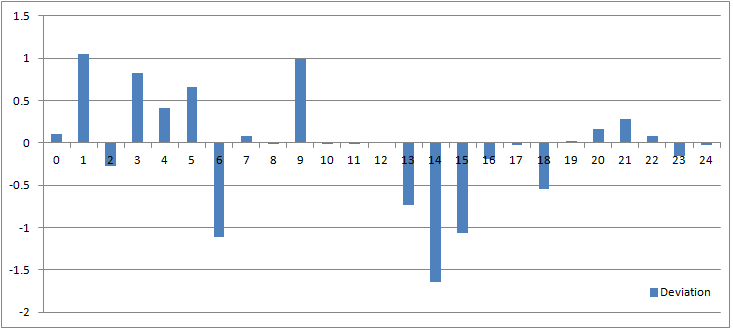
\includegraphics[width=0.7\linewidth]{../NodeDeviations/Ariadne60}
\caption{Total interaction shift by node for Ariadne (60km).}
\label{fig:Ariadne60}
\end{figure}

\begin{figure}[H]
\centering
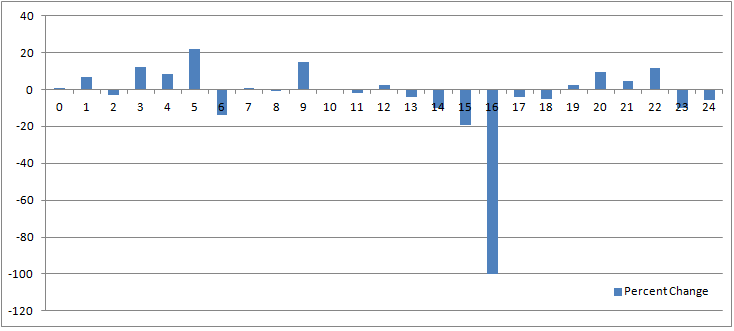
\includegraphics[width=0.7\linewidth]{../NodeDeviations/AriadnePercent60}
\caption{Percent total interaction shift by node for Ariadne (60km).}
\label{fig:AriadnePercent60}
\end{figure}

\begin{figure}[H]
\centering
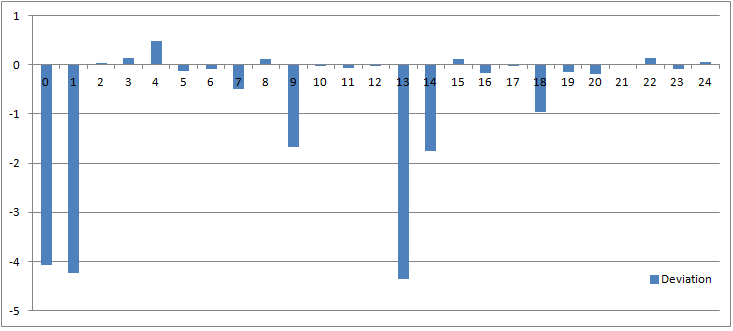
\includegraphics[width=0.7\linewidth]{../NodeDeviations/Ariadne100}
\caption{Total interaction shift by node for Ariadne (100km).}
\label{fig:Ariadne100}
\end{figure}

\begin{figure}[H]
\centering
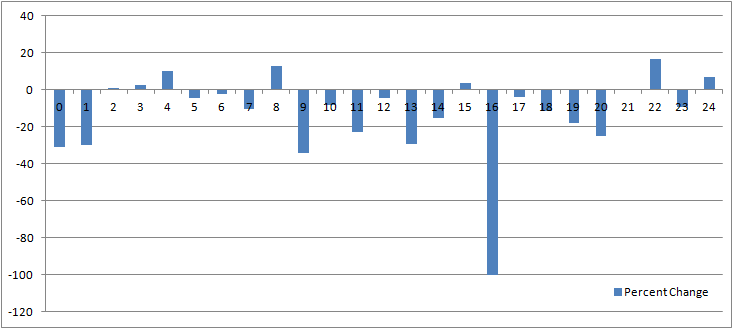
\includegraphics[width=0.7\linewidth]{../NodeDeviations/AriadnePercent100}
\caption{Percent total interaction shift by node for Ariadne (100km).}
\label{fig:AriadnePercent100}
\end{figure}



\section{Agent-based Model}

\paragraph{}
Similarly, the agent-based model network-level metric results converged to steady values within 25 models runs. While Poggio Civitate does not appear to be highly connected it does seem to be central to the northern settlements. On average the model results suggest that Murlo would have maintained 2-3 incoming edges and about 3 outgoing edges. Though the agent-based model has produced the most promising evidence for Murlo as a central node the interaction quantity maintained over its edges would still have been among the weakest within the system. Even if Poggio Civitate did sustain connections with as many as six other settlements it was likely not fostering strong affiliations. PageRank and HITS values are very small and therefore do not indicate that Murlo was serving an important central function.

\paragraph{}
Visually, the networks from this model seem to be resulting in communities with higher connectivities. Transitivity values show that there is some association between neighbors. Overall, these networks are less connected than previous models, which is supported by a smaller average degree. The removal of Murlo does not seem to suggest any strong fluctuations within the system. Minor decreases in the average degree and beta index suggest slightly less connectivity while small increases in the gamma index suggest higher connectivity. All of these variations are small and do not provide strong evidence towards any real transformations of the network. Similar to the Ariadne results the mixed evidence is likely due to noise generated from the stochastic nature of the model. Individual nodes are split between interaction gains and loses and most variations occurring at less than 10 percent deviations. Nodes 18, 19, and 20 show moderate increases around 15-20 percent while node 24 shows intense gains of about 50 percent. Likewise, 7 and 11 have the highest loses which approaches 20 percent. 

\subsubsection{Before}

\begin{figure}[H]
\centering
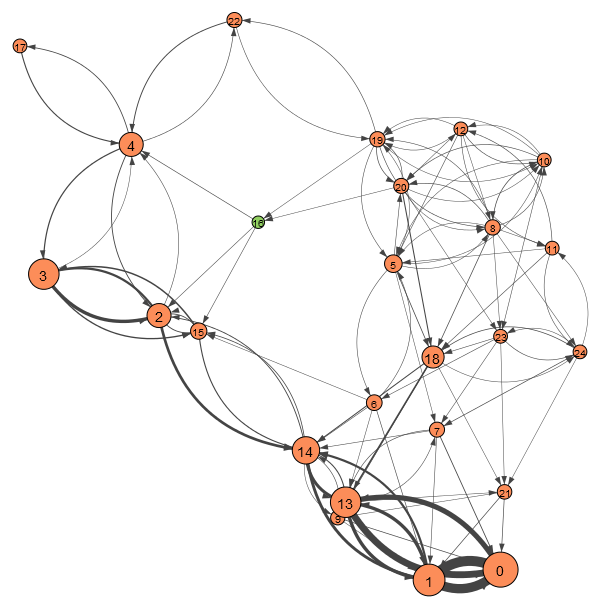
\includegraphics[width=0.35\linewidth]{./BeforeViz/agent}
\caption{Visualization of a single agent-based model run including Murlo.}
\label{fig:agentBefore}
\end{figure}

\begin{figure}[H]
\centering
\tiny
\begin{tabular}{|c|c|c|c|c|c|c|}
\hline Metric & Assortativity & Diameter & Average Degree & Transitivity & Beta & Gamma \\ 
\hline Agent Model (Before) & -0.03900133 & 5.0	& 8.3136 & 0.43295384 & 4.1568	& 0.166272 \\ 
\hline 
\end{tabular} 
\end{figure}

\begin{figure}[H]
\centering
\tiny
\begin{tabular}{|c|c|c|c|c|c|c|c|}
\hline	Node	&	Interaction In	&	Interaction Out	&	Degree In	&	Degree Out	&	PageRank	&	Hubs	&	Authorities	\\
\hline	0	&	268.8800	&	235.3600	&	5.0000	&	3.5200	&	0.20116159	&	0.27213437	&	0.35633480	\\
\hline	1	&	252.7200	&	222.3600	&	7.0000	&	4.2800	&	0.18596166	&	0.28471034	&	0.29682130	\\
\hline	2	&	84.6000	&	87.0000	&	5.0000	&	4.2400	&	0.05479031	&	0.00688518	&	0.00568801	\\
\hline	3	&	73.8400	&	77.1200	&	3.0000	&	3.0000	&	0.04913631	&	0.00196484	&	0.00214724	\\
\hline	4	&	26.9200	&	31.9200	&	5.0000	&	4.1600	&	0.02688070	&	0.00030261	&	0.00009308	\\
\hline	5	&	12.9600	&	17.9600	&	5.8000	&	5.7200	&	0.01715167	&	0.00009261	&	0.00012245	\\
\hline	6	&	10.3200	&	15.3200	&	2.4400	&	5.1600	&	0.01464954	&	0.01140266	&	0.00029078	\\
\hline	7	&	9.1200	&	13.8800	&	4.0400	&	4.2000	&	0.01425532	&	0.01648979	&	0.00502421	\\
\hline	8	&	7.5600	&	12.5200	&	3.4000	&	5.4800	&	0.01281434	&	0.00000104	&	0.00000039	\\
\hline	9	&	24.2400	&	26.8000	&	5.6000	&	4.0400	&	0.02329927	&	0.03309842	&	0.02744999	\\
\hline	10	&	5.5200	&	10.5200	&	3.0800	&	4.7600	&	0.01080427	&	0.00000177	&	0.00000036	\\
\hline	11	&	5.7600	&	10.7200	&	3.2000	&	4.4000	&	0.01145565	&	0.00000112	&	0.00000585	\\
\hline	12	&	6.0400	&	10.8800	&	3.1600	&	4.0000	&	0.01133522	&	0.00000173	&	0.00000011	\\
\hline	13	&	223.5600	&	194.9200	&	7.6000	&	6.0000	&	0.16549250	&	0.25261614	&	0.26289842	\\
\hline	14	&	85.5600	&	86.4800	&	8.0000	&	5.4000	&	0.06104593	&	0.08582814	&	0.03723831	\\
\hline	15	&	32.0400	&	36.2800	&	4.5200	&	3.2000	&	0.02433631	&	0.00220370	&	0.00178417	\\
\hline	16	&	3.6800	&	8.6800	&	2.5200	&	3.1600	&	0.00896006	&	0.00011064	&	0.00001616	\\
\hline	17	&	5.7600	&	10.7600	&	1.0000	&	1.0000	&	0.01010698	&	0.00000425	&	0.00000882	\\
\hline	18	&	20.9600	&	25.9600	&	5.8000	&	4.8000	&	0.02543693	&	0.01577961	&	0.00001974	\\
\hline	19	&	7.8800	&	12.8000	&	3.5200	&	5.6800	&	0.01263052	&	0.00000167	&	0.00000015	\\
\hline	20	&	7.2000	&	12.1600	&	3.8000	&	4.8000	&	0.01221435	&	0.00000113	&	0.00001020	\\
\hline	21	&	7.1600	&	11.9200	&	4.1200	&	2.8000	&	0.01275270	&	0.01624084	&	0.00398420	\\
\hline	22	&	7.9200	&	12.8800	&	2.0000	&	2.0000	&	0.01208800	&	0.00000397	&	0.00000625	\\
\hline	23	&	4.9600	&	9.9600	&	3.1200	&	5.1200	&	0.01091704	&	0.00007750	&	0.00001999	\\
\hline	24	&	4.8400	&	4.8400	&	2.2000	&	3.0000	&	0.01032283	&	0.00004596	&	0.00003502	\\
\hline 
\end{tabular} 
\end{figure}

\subsubsection{After}

\begin{figure}[H]
\centering
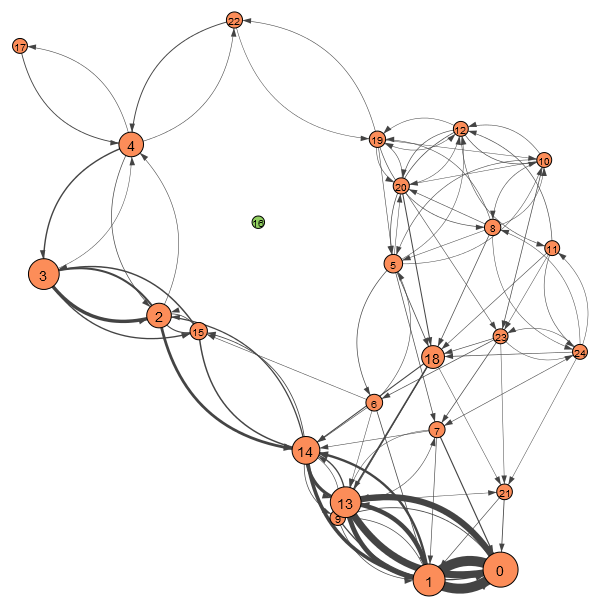
\includegraphics[width=0.35\linewidth]{./AfterViz/agent}
\caption{Visualization of a single agent-based model run excluding Murlo.}
\label{fig:agentAfter}
\end{figure}

\begin{figure}[H]
\centering
\tiny
\begin{tabular}{|c|c|c|c|c|c|c|}
\hline Metric & Assortativity & Diameter & Average Degree & Transitivity & Beta & Gamma \\ 
\hline Agent Model (After) & -0.02370421 & 5.0 & 7.9744 & 0.44168669 & 4.15333333 & 0.17305556 \\ 
\hline 
\end{tabular} 
\end{figure}

\begin{figure}[H]
\centering
\tiny
\begin{tabular}{|c|c|c|c|c|c|c|c|}
\hline	Node	&	Interaction In	&	Interaction Out	&	Degree In	&	Degree Out	&	PageRank	&	Hubs	&	Authorities	\\
\hline	0	&	276.0400	&	242.0000	&	5.0000	&	2.9200 &	0.20667059	&	0.27516427	&	0.35770363	\\
\hline	1	&	254.9600	&	223.4800	&	7.0000	&	3.8400	&	0.18786417	&	0.28145215	&	0.29851473	\\
\hline	2	&	73.8800	&	77.5600	&	4.0000	&	4.0000	&	0.04860014	&	0.00605907	&	0.00559860	\\
\hline	3	&	64.0800	&	68.3600	&	3.0000	&	3.0000	&	0.04413701	&	0.00148406	&	0.00142513	\\
\hline	4	&	27.6400	&	32.4800	&	4.0000	&	4.0000	&	0.02751972	&	0.00025992	&	0.00009594	\\
\hline	5	&	12.8800	&	17.8800	&	6.0400	&	5.3200	&	0.01752550	&	0.00003045	&	0.00013090	\\
\hline	6	&	11.6800	&	16.6800	&	2.2000	&	5.2000	&	0.01611379	&	0.01251641	&	0.00054420	\\
\hline	7	&	7.1600	&	12.1600	&	3.6400	&	4.1200	&	0.01230714	&	0.01444776	&	0.00272638	\\
\hline	8	&	8.4800	&	13.3600	&	4.0400	&	5.0000	&	0.01372132	&	0.00000107	&	0.00000038	\\
\hline	9	&	26.7600	&	28.7600	&	5.0800	&	4.0800	&	0.02518492	&	0.03464417	&	0.02987861	\\
\hline	10	&	6.2800	&	11.2400	&	3.4000	&	4.8400	&	0.01175978	&	0.00000163	&	0.00000024	\\
\hline	11	&	4.2400	&	9.2400	&	2.6400	&	4.4400	&	0.01008040	&	0.00000061	&	0.00000030	\\
\hline	12	&	5.8000	&	10.7600	&	3.0000	&	4.5200	&	0.01139420	&	0.00000154	&	0.00000015	\\
\hline	13	&	230.8400	&	200.4000	&	7.6400	&	5.8800	&	0.17007393	&	0.25537514	&	0.26237901	\\
\hline	14	&	86.3200	&	88.5600	&	8.0000	&	5.0000	&	0.06153044	&	0.08244504	&	0.03534963	\\
\hline	15	&	29.1600	&	33.7200	&	3.8400	&	3.0400	&	0.02266485	&	0.00209317	&	0.00221989	\\
\hline	16	&	0.0000	&	0.0000	&	999	&	999	&	999	&	999	&	999	\\
\hline	17	&	6.0800	&	11.0800	&	1.0000	&	1.0000	&	0.01065550	&	0.00000445	&	0.00000777	\\
\hline	18	&	24.3200	&	29.3200	&	6.0000	&	4.5200	&	0.02741361	&	0.01860784	&	0.00000198	\\
\hline	19	&	9.6400	&	14.4800	&	4.1600	&	4.7200	&	0.01456341	&	0.00000150	&	0.00000011	\\
\hline	20	&	9.3200	&	14.3200	&	4.8400	&	4.6000	&	0.01433156	&	0.00000092	&	0.00001689	\\
\hline	21	&	6.5600	&	11.3600	&	4.2000	&	2.8800	&	0.01171616	&	0.01529332	&	0.00336850	\\
\hline	22	&	8.1600	&	13.0800	&	2.0000	&	1.8000	&	0.01293553	&	0.00000434	&	0.00000313	\\
\hline	23	&	4.8400	&	9.8400	&	2.7200	&	5.5600	&	0.01060208	&	0.00006222	&	0.00000047	\\
\hline	24	&	4.8800	&	9.8800	&	2.2400	&	5.4000	&	0.01063426	&	0.00004895	&	0.00003342	\\
\hline
\end{tabular} 
\end{figure}

\subsubsection{Interaction Shifts}

\begin{figure}[H]
\centering
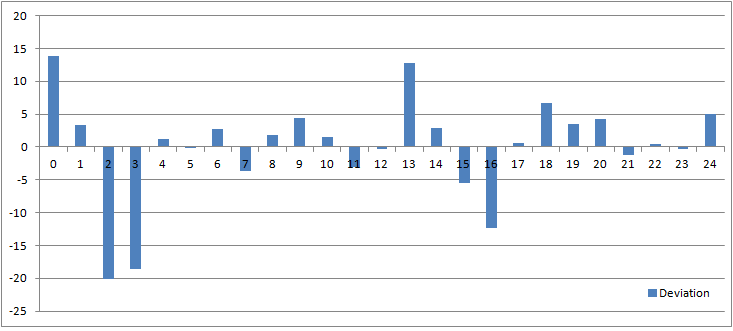
\includegraphics[width=0.7\linewidth]{../NodeDeviations/Agent}
\caption{Total interaction shift by node for agent-based model.}
\label{fig:Agent}
\end{figure}

\begin{figure}[H]
\centering
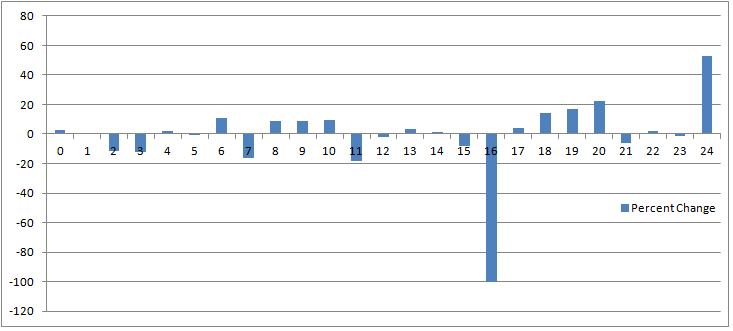
\includegraphics[width=0.7\linewidth]{../NodeDeviations/AgentPercent}
\caption{Percent total interaction shift by node for agent-based model.}
\label{fig:AgentPercent}
\end{figure}



\chapter{Discussion}
\section{Implications for Poggio Civitate and Etruria}
\paragraph{}
None of the models in this research indicate that Poggio Civitate was a highly connected central node within a larger network. Only within the context of the agent-based model did this geographically centrally located settlement command mild network centrality and even then it was not enough to drastically alter the network once the site was destroyed. It is therefore important to differentiate between these two concepts. Given Murlo's size and the collective distances required to travel to other settlements it is highly unlikely that it leveraged any natural geographic advantages. Individual node metrics such as PageRank and HITS did not show any signs that Poggio Civitate was punching above its weight and therefore maintained high levels of interaction despite its relatively smaller size. Instead, it seems probable that the elite society which dwelt upon the hilltop site enjoyed relative autonomy. 
\paragraph{}
In every model the connections Murlo held with other settlements was always among the weakest levels in interactions throughout the system and would be representative of loose affiliations. Those in control could have exploited these limited relationships in order to grow their authority and power. It is also clear that the distances prescribed within the models to differentiate between walking and horseback transportation will give different results. The agent-based model suggests those limited to walking would have been at a severe disadvantage for participating in the wider network, especially in the north. Similarly, the Ariadne networks with higher distance thresholds (100km) resulted in higher connectivity. If access to horses can be seen as a luxury only for those with elite status than it is also possible to differentiate between varying interaction networks within a society depending on social hierarchy. Moreover, the Ariadne results suggest that networks governed less by spatial restrictions may have been less resilient and that removing nodes could have a larger impact on overall interaction sustainability. Arguably, the total decrease in interaction could call for a complete system shift which would require model parameter changes that result in a much less connected network similar to the research completed concerning Thera in the Greek Mediterranean during the Bronze Age \citeyearpar{KnaRivEva11}.      

\paragraph{}
It is intriguing that in two different scenarios (radiation model and Ariadne (60km)) node number 5 (Chiusi) gained significant interaction increases. This provides initial evidence towards a motive for the destruction of Murlo. In order to further test the theory that Chiusi eliminated the society at Poggio Civitate in order to better situate itself in the regional network it will be necessary to continue testing the stochastic models and collect further results. It would also be interesting to observe whether or not patterns emerge suggesting relationships between Poggio Civitate's demise and any other settlement's rise.
  

\section{Comparing and Contrasting the Models}
\paragraph{}
Each model used in this research returned spatial interaction networks which were similar in their general structure. This suggests that their was certainly a spatial component to each model that was successfully being captured. Nevertheless, the different analytical frameworks produced unique results each with their own characteristics.  

-Assortativity

\section{Limitations - Future Work}
-filtering
-agent model should have considered starting agent populations in proportion to starting size
-change importance calculation to be local (iteration) rather than global (entire simulation) the number of visitors
-data limitations


\chapter{Conclusion}

\begin{singlespace}
\bibliographystyle{apa-good}
\bibliography{bibfile}
\end{singlespace}

{\newgeometry{left=1.4in,right=.75in,top=1in,bottom=1in, includehead, includefoot}
\begin{appendices}
\restoregeometry
\chapter{}

\begin{figure}
\centering
\includegraphics[width=0.7\linewidth]{../SlopeReclass}
\caption{Study region slope reclassified according to energy costs.}
\label{fig:slopeReclass}
\end{figure}



\begin{sidewaystable}
\centering
\tiny
\begin{tabular}{|c|c|c|c|c|c|c|c|c|c|c|c|c|c|c|c|c|c|c|c|c|c|c|c|c|c|}
\hline	-	&	0	&	1	&	2	&	3	&	4	&	5	&	6	&	7	&	8	&	9	&	10	&	11	&	12	&	13	&	14	&	15	&	16	&	17	&	18	&	19	&	20	&	21	&	22	&	23	&	24	\\
\hline	0	&	0	&	36	&	211	&	274	&	282	&	170	&	105	&	80	&	172	&	87	&	211	&	167	&	227	&	86	&	115	&	190	&	217	&	354	&	116	&	234	&	207	&	39	&	321	&	119	&	123	\\
\hline	1	&	36	&	0	&	185	&	244	&	272	&	162	&	97	&	75	&	185	&	55	&	228	&	185	&	232	&	57	&	89	&	168	&	207	&	343	&	112	&	227	&	199	&	57	&	313	&	133	&	142	\\
\hline	2	&	211	&	185	&	0	&	63	&	91	&	120	&	119	&	153	&	175	&	134	&	213	&	198	&	181	&	128	&	97	&	22	&	68	&	161	&	137	&	139	&	140	&	197	&	161	&	168	&	210	\\
\hline	3	&	274	&	244	&	63	&	0	&	83	&	168	&	181	&	216	&	221	&	191	&	259	&	245	&	227	&	189	&	161	&	84	&	112	&	122	&	199	&	184	&	186	&	260	&	165	&	228	&	271	\\
\hline	4	&	282	&	272	&	91	&	83	&	0	&	147	&	179	&	209	&	186	&	223	&	205	&	218	&	165	&	217	&	185	&	106	&	75	&	74	&	186	&	120	&	135	&	254	&	83	&	212	&	253	\\
\hline	5	&	170	&	162	&	120	&	168	&	147	&	0	&	72	&	90	&	54	&	135	&	94	&	77	&	81	&	126	&	108	&	105	&	72	&	220	&	53	&	65	&	40	&	133	&	152	&	66	&	106	\\
\hline	6	&	105	&	97	&	119	&	181	&	179	&	72	&	0	&	35	&	109	&	63	&	153	&	117	&	152	&	54	&	42	&	97	&	112	&	252	&	37	&	134	&	112	&	79	&	216	&	73	&	108	\\
\hline	7	&	80	&	75	&	153	&	216	&	209	&	90	&	35	&	0	&	110	&	64	&	153	&	112	&	158	&	57	&	65	&	132	&	137	&	282	&	38	&	154	&	127	&	45	&	241	&	59	&	85	\\
\hline	8	&	172	&	185	&	175	&	221	&	186	&	54	&	109	&	110	&	0	&	172	&	44	&	33	&	55	&	163	&	147	&	159	&	113	&	258	&	75	&	81	&	52	&	132	&	169	&	55	&	78	\\
\hline	9	&	87	&	55	&	134	&	191	&	223	&	135	&	63	&	64	&	172	&	0	&	215	&	175	&	215	&	9	&	39	&	118	&	160	&	293	&	97	&	193	&	174	&	83	&	266	&	122	&	149	\\
\hline	10	&	211	&	228	&	213	&	259	&	205	&	94	&	153	&	153	&	44	&	215	&	0	&	47	&	46	&	206	&	190	&	198	&	148	&	271	&	119	&	86	&	74	&	171	&	177	&	96	&	103	\\
\hline	11	&	167	&	185	&	198	&	245	&	218	&	77	&	117	&	112	&	33	&	175	&	47	&	0	&	77	&	167	&	158	&	182	&	143	&	290	&	81	&	109	&	84	&	129	&	200	&	54	&	56	\\
\hline	12	&	227	&	232	&	181	&	227	&	165	&	81	&	152	&	158	&	55	&	215	&	46	&	77	&	0	&	206	&	189	&	167	&	116	&	225	&	121	&	45	&	45	&	187	&	131	&	110	&	132	\\
\hline	13	&	86	&	57	&	128	&	189	&	217	&	126	&	54	&	57	&	163	&	9	&	206	&	167	&	206	&	0	&	33	&	112	&	154	&	287	&	88	&	185	&	165	&	77	&	260	&	113	&	142	\\
\hline	14	&	115	&	89	&	97	&	161	&	185	&	108	&	42	&	65	&	147	&	39	&	190	&	158	&	189	&	33	&	0	&	79	&	121	&	255	&	78	&	167	&	148	&	101	&	227	&	115	&	150	\\
\hline	15	&	190	&	168	&	22	&	84	&	106	&	105	&	97	&	132	&	159	&	118	&	198	&	182	&	167	&	112	&	79	&	0	&	65	&	176	&	117	&	131	&	125	&	176	&	163	&	149	&	190	\\
\hline	16	&	217	&	207	&	68	&	112	&	75	&	72	&	112	&	137	&	113	&	160	&	148	&	143	&	116	&	154	&	121	&	65	&	0	&	148	&	111	&	73	&	74	&	181	&	107	&	137	&	178	\\
\hline	17	&	354	&	343	&	161	&	122	&	74	&	220	&	252	&	282	&	258	&	293	&	271	&	290	&	225	&	287	&	255	&	176	&	148	&	0	&	258	&	188	&	207	&	326	&	106	&	285	&	325	\\
\hline	18	&	116	&	112	&	137	&	199	&	186	&	53	&	37	&	38	&	75	&	97	&	119	&	81	&	121	&	88	&	78	&	117	&	111	&	258	&	0	&	118	&	90	&	80	&	205	&	37	&	75	\\
\hline	19	&	234	&	227	&	139	&	184	&	120	&	65	&	134	&	154	&	81	&	193	&	86	&	109	&	45	&	185	&	167	&	131	&	73	&	188	&	118	&	0	&	28	&	198	&	94	&	121	&	150	\\
\hline	20	&	207	&	199	&	140	&	186	&	135	&	40	&	112	&	127	&	52	&	174	&	74	&	84	&	45	&	165	&	148	&	125	&	74	&	207	&	90	&	28	&	0	&	170	&	116	&	93	&	122	\\
\hline	21	&	39	&	57	&	197	&	260	&	254	&	133	&	79	&	45	&	132	&	83	&	171	&	129	&	187	&	77	&	101	&	176	&	181	&	326	&	80	&	198	&	170	&	0	&	285	&	79	&	85	\\
\hline	22	&	321	&	313	&	161	&	165	&	83	&	152	&	216	&	241	&	169	&	266	&	177	&	200	&	131	&	260	&	227	&	163	&	107	&	106	&	205	&	94	&	116	&	285	&	0	&	209	&	238	\\
\hline	23	&	119	&	133	&	168	&	228	&	212	&	66	&	73	&	59	&	55	&	122	&	96	&	54	&	110	&	113	&	115	&	149	&	137	&	285	&	37	&	121	&	93	&	79	&	209	&	0	&	41	\\
\hline	24	&	123	&	142	&	210	&	271	&	253	&	106	&	108	&	85	&	78	&	149	&	103	&	56	&	132	&	142	&	150	&	190	&	178	&	325	&	75	&	150	&	122	&	85	&	238	&	41	&	0	\\
\hline
\end{tabular}
\caption{Least-cost path distances (km)} 
\label{fig:LCP}
\end{sidewaystable}


\begin{sidewaystable}
\centering
\tiny
\begin{tabular}{|c|c|c|c|c|c|c|c|c|c|c|c|c|c|c|c|c|c|c|c|c|c|c|c|c|c|}
\hline	-	&	0	&	1	&	2	&	3	&	4	&	5	&	6	&	7	&	8	&	9	&	10	&	11	&	12	&	13	&	14	&	15	&	16	&	17	&	18	&	19	&	20	&	21	&	22	&	23	&	24	\\
\hline	0	&	0	&	34	&	202	&	257	&	270	&	157	&	100	&	74	&	166	&	80	&	200	&	158	&	216	&	79	&	108	&	182	&	203	&	340	&	108	&	217	&	192	&	38	&	296	&	113	&	112	\\
\hline	1	&	34	&	0	&	180	&	233	&	254	&	154	&	90	&	73	&	174	&	52	&	211	&	171	&	220	&	54	&	85	&	162	&	191	&	323	&	108	&	216	&	192	&	55	&	288	&	123	&	131	\\
\hline	2	&	202	&	180	&	0	&	58	&	85	&	112	&	109	&	141	&	162	&	129	&	195	&	187	&	168	&	126	&	95	&	20	&	65	&	148	&	130	&	134	&	130	&	183	&	150	&	160	&	197	\\
\hline	3	&	257	&	233	&	58	&	0	&	76	&	163	&	167	&	199	&	211	&	181	&	240	&	238	&	207	&	179	&	150	&	78	&	103	&	113	&	186	&	169	&	172	&	240	&	154	&	216	&	253	\\
\hline	4	&	270	&	254	&	85	&	76	&	0	&	136	&	170	&	200	&	174	&	206	&	193	&	203	&	154	&	201	&	170	&	97	&	71	&	71	&	175	&	115	&	128	&	243	&	78	&	196	&	233	\\
\hline	5	&	157	&	154	&	112	&	163	&	136	&	0	&	68	&	83	&	50	&	126	&	87	&	75	&	73	&	118	&	100	&	97	&	66	&	205	&	49	&	62	&	38	&	123	&	141	&	61	&	97	\\
\hline	6	&	100	&	90	&	109	&	167	&	170	&	68	&	0	&	32	&	102	&	58	&	143	&	112	&	140	&	50	&	39	&	89	&	103	&	241	&	35	&	129	&	107	&	75	&	199	&	67	&	99	\\
\hline	7	&	74	&	73	&	141	&	199	&	200	&	83	&	32	&	0	&	102	&	63	&	141	&	104	&	147	&	55	&	62	&	121	&	131	&	271	&	35	&	145	&	120	&	44	&	222	&	54	&	77	\\
\hline	8	&	166	&	174	&	162	&	211	&	174	&	50	&	102	&	102	&	0	&	159	&	41	&	30	&	51	&	150	&	139	&	146	&	110	&	238	&	69	&	69	&	47	&	129	&	158	&	53	&	73	\\
\hline	9	&	80	&	52	&	129	&	181	&	206	&	126	&	58	&	63	&	159	&	0	&	199	&	165	&	198	&	8	&	36	&	111	&	149	&	274	&	90	&	186	&	164	&	79	&	248	&	116	&	139	\\
\hline	10	&	200	&	211	&	195	&	240	&	193	&	87	&	143	&	141	&	41	&	199	&	0	&	43	&	42	&	191	&	180	&	182	&	137	&	251	&	110	&	79	&	68	&	163	&	160	&	89	&	95	\\
\hline	11	&	158	&	171	&	187	&	238	&	203	&	75	&	112	&	104	&	30	&	165	&	43	&	0	&	72	&	157	&	151	&	170	&	138	&	268	&	77	&	98	&	77	&	121	&	186	&	49	&	52	\\
\hline	12	&	216	&	220	&	168	&	207	&	154	&	73	&	140	&	147	&	51	&	198	&	42	&	72	&	0	&	190	&	173	&	158	&	105	&	210	&	113	&	39	&	40	&	178	&	119	&	103	&	123	\\
\hline	13	&	79	&	54	&	126	&	179	&	201	&	118	&	50	&	55	&	150	&	8	&	191	&	157	&	190	&	0	&	31	&	108	&	142	&	270	&	81	&	178	&	156	&	74	&	242	&	108	&	132	\\
\hline	14	&	108	&	85	&	95	&	150	&	170	&	100	&	39	&	62	&	139	&	36	&	180	&	151	&	173	&	31	&	0	&	77	&	113	&	239	&	75	&	156	&	137	&	95	&	214	&	106	&	137	\\
\hline	15	&	182	&	162	&	20	&	78	&	97	&	97	&	89	&	121	&	146	&	111	&	182	&	170	&	158	&	108	&	77	&	0	&	60	&	163	&	110	&	126	&	118	&	163	&	154	&	141	&	178	\\
\hline	16	&	203	&	191	&	65	&	103	&	71	&	66	&	103	&	131	&	110	&	149	&	137	&	138	&	105	&	142	&	113	&	60	&	0	&	141	&	105	&	69	&	69	&	175	&	100	&	126	&	163	\\
\hline	17	&	340	&	323	&	148	&	113	&	71	&	205	&	241	&	271	&	238	&	274	&	251	&	268	&	210	&	270	&	239	&	163	&	141	&	0	&	246	&	173	&	191	&	314	&	101	&	266	&	302	\\
\hline	18	&	108	&	108	&	130	&	186	&	175	&	49	&	35	&	35	&	69	&	90	&	110	&	77	&	113	&	81	&	75	&	110	&	105	&	246	&	0	&	110	&	85	&	73	&	190	&	33	&	69	\\
\hline	19	&	217	&	216	&	134	&	169	&	115	&	62	&	129	&	145	&	69	&	186	&	79	&	98	&	39	&	178	&	156	&	126	&	69	&	173	&	110	&	0	&	26	&	182	&	89	&	112	&	141	\\
\hline	20	&	192	&	192	&	130	&	172	&	128	&	38	&	107	&	120	&	47	&	164	&	68	&	77	&	40	&	156	&	137	&	118	&	69	&	191	&	85	&	26	&	0	&	157	&	113	&	87	&	116	\\
\hline	21	&	38	&	55	&	183	&	240	&	243	&	123	&	75	&	44	&	129	&	79	&	163	&	121	&	178	&	74	&	95	&	163	&	175	&	314	&	73	&	182	&	157	&	0	&	263	&	76	&	77	\\
\hline	22	&	296	&	288	&	150	&	154	&	78	&	141	&	199	&	222	&	158	&	248	&	160	&	186	&	119	&	242	&	214	&	154	&	100	&	101	&	190	&	89	&	113	&	263	&	0	&	199	&	229	\\
\hline	23	&	113	&	123	&	160	&	216	&	196	&	61	&	67	&	54	&	53	&	116	&	89	&	49	&	103	&	108	&	106	&	141	&	126	&	266	&	33	&	112	&	87	&	76	&	199	&	0	&	38	\\
\hline	24	&	112	&	131	&	197	&	253	&	233	&	97	&	99	&	77	&	73	&	139	&	95	&	52	&	123	&	132	&	137	&	178	&	163	&	302	&	69	&	141	&	116	&	77	&	229	&	38	&	0	\\
\hline
\end{tabular}
\caption{As the crow flies distances (km)} 
\label{fig:crowDist}
\end{sidewaystable}



\begin{figure}
\centering
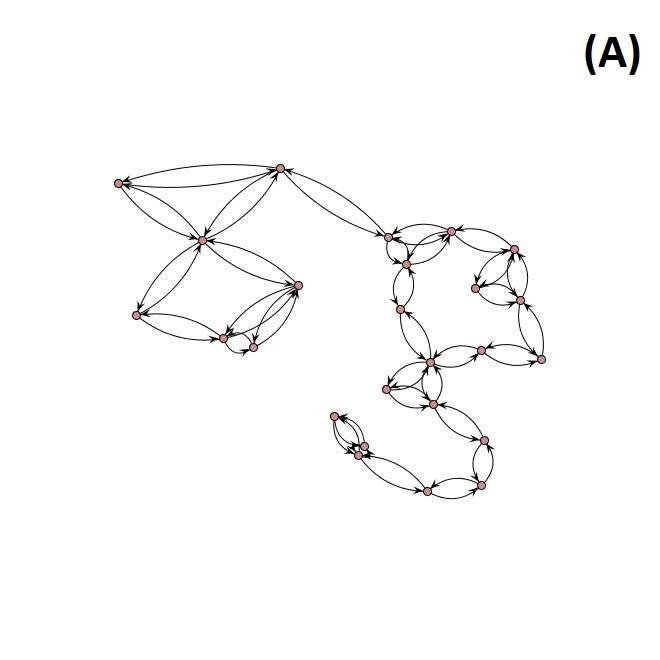
\includegraphics[width=0.3\linewidth]{../ExploratoryModelAnalysis/PPA/lcptest_PPA-beta001_r0_sl50_j0}
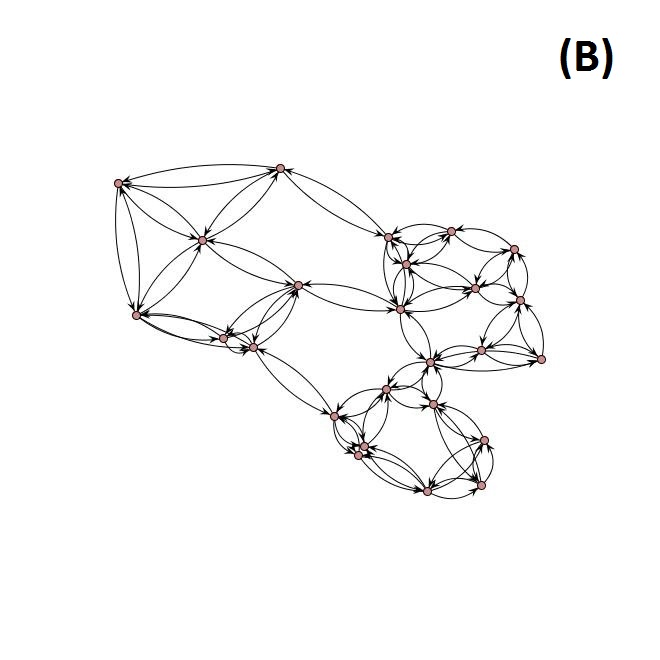
\includegraphics[width=0.3\linewidth]{../ExploratoryModelAnalysis/PPA/lcptest_PPA-beta002_r0_sl50_j0}
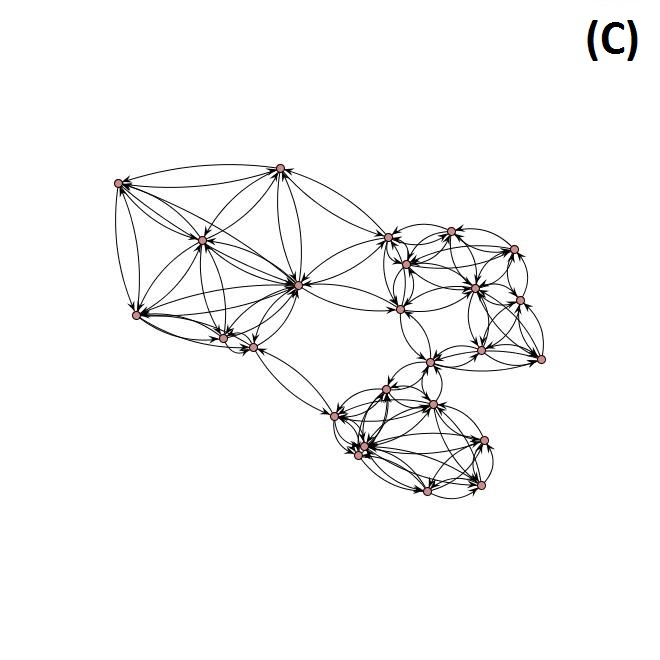
\includegraphics[width=0.3\linewidth]{../ExploratoryModelAnalysis/PPA/lcptest_PPA-beta003_r0_sl50_j0}
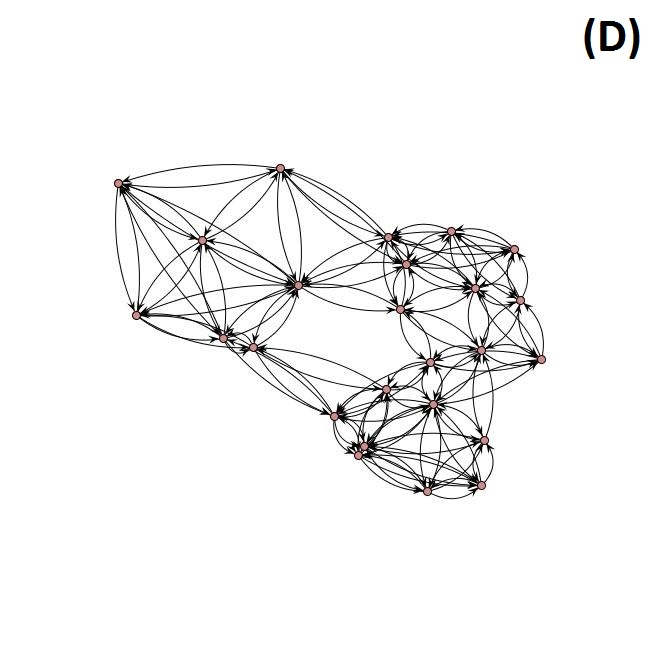
\includegraphics[width=0.3\linewidth]{../ExploratoryModelAnalysis/PPA/lcptest_PPA-beta004_r0_sl50_j0}
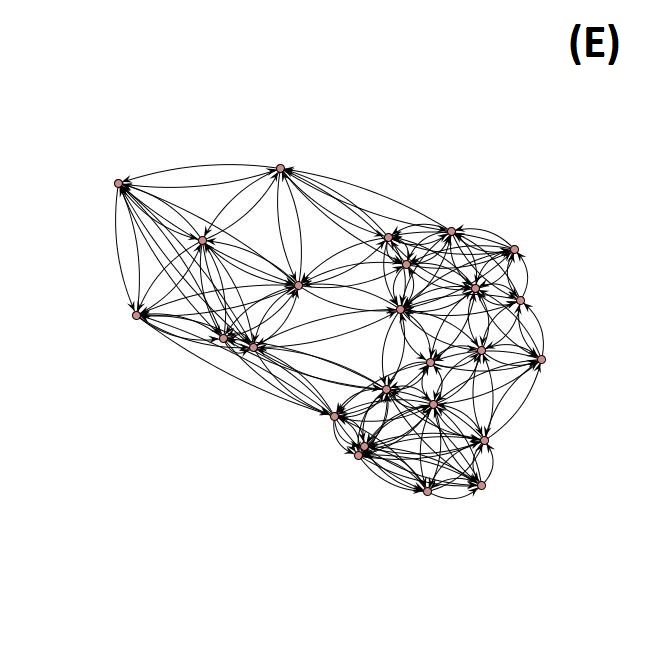
\includegraphics[width=0.3\linewidth]{../ExploratoryModelAnalysis/PPA/lcptest_PPA-beta005_r0_sl50_j0}
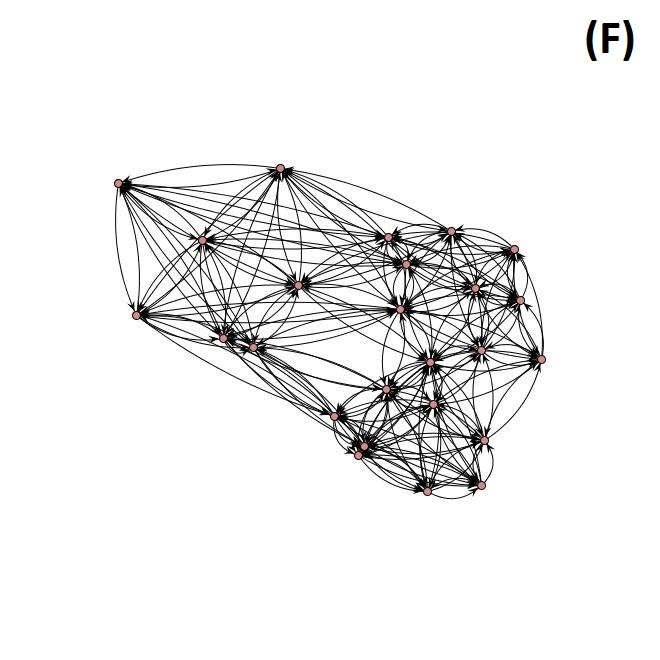
\includegraphics[width=0.3\linewidth]{../ExploratoryModelAnalysis/PPA/lcptest_PPA-beta007_r0_sl50_j0}
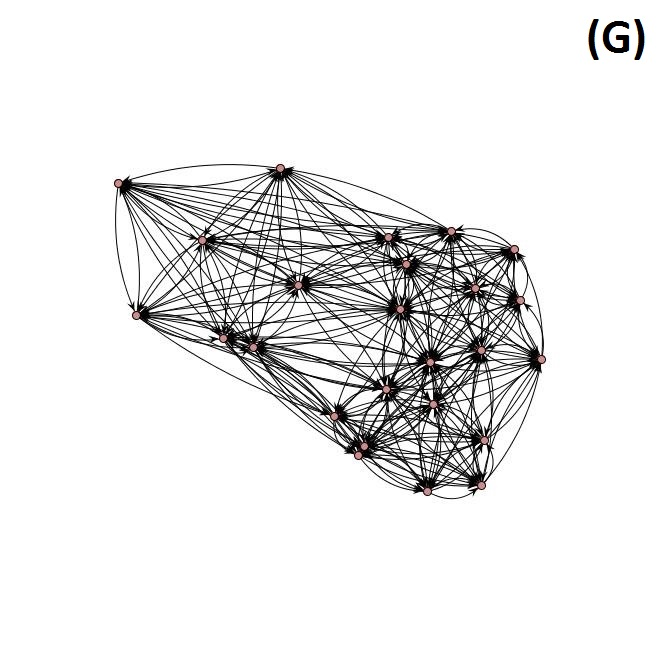
\includegraphics[width=0.3\linewidth]{../ExploratoryModelAnalysis/PPA/lcptest_PPA-beta009_r0_sl50_j0}
\caption{A-G: PPA results for $k$ equals 1, 2, 3, 4, 5, 7, and 9.}
\label{fig:PPA}
\end{figure}

\begin{figure}
\centering
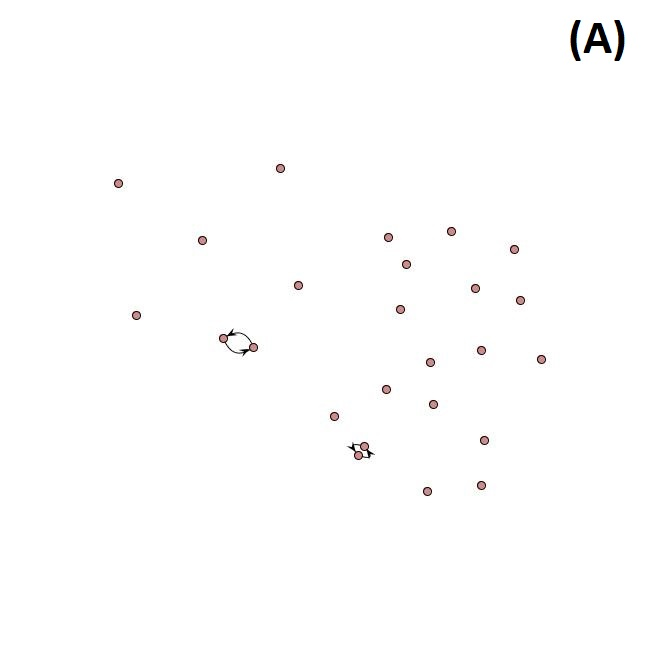
\includegraphics[width=0.3\linewidth]{../ExploratoryModelAnalysis/MDN/lcptest_MDN-D25_r0_sl50_j0}
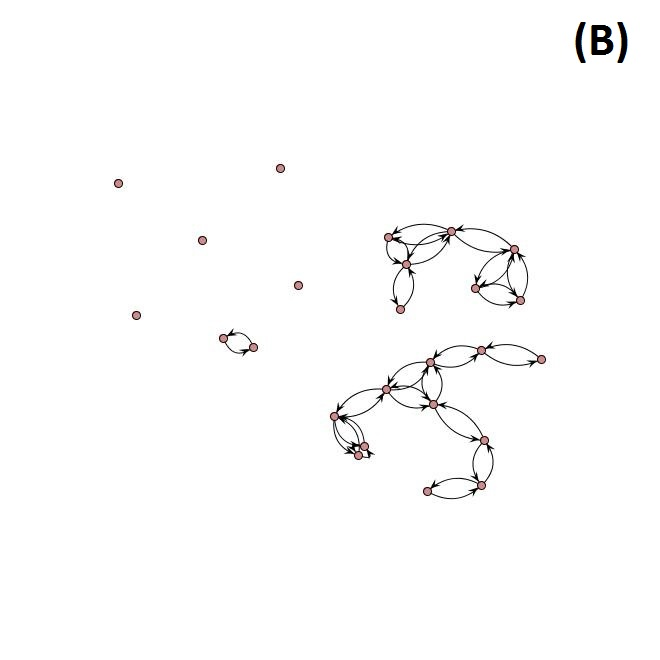
\includegraphics[width=0.3\linewidth]{../ExploratoryModelAnalysis/MDN/lcptest_MDN-D50_r0_sl50_j0}
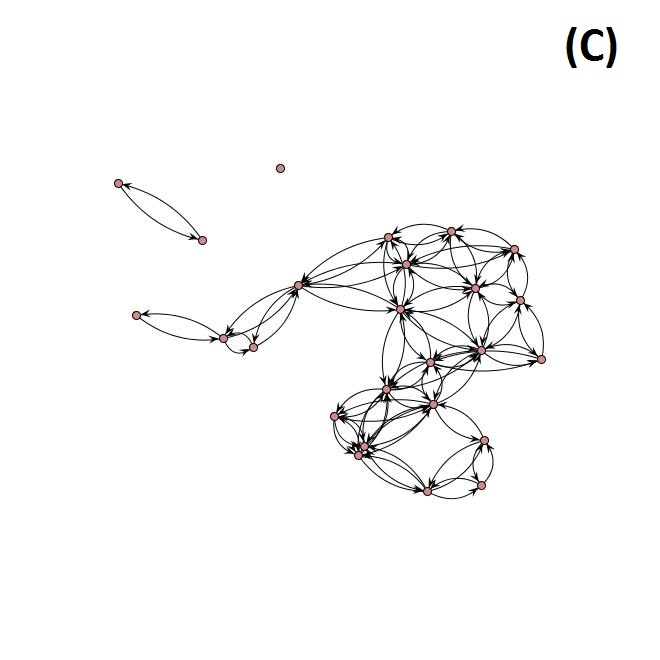
\includegraphics[width=0.3\linewidth]{../ExploratoryModelAnalysis/MDN/lcptest_MDN-D75_r0_sl50_j0}
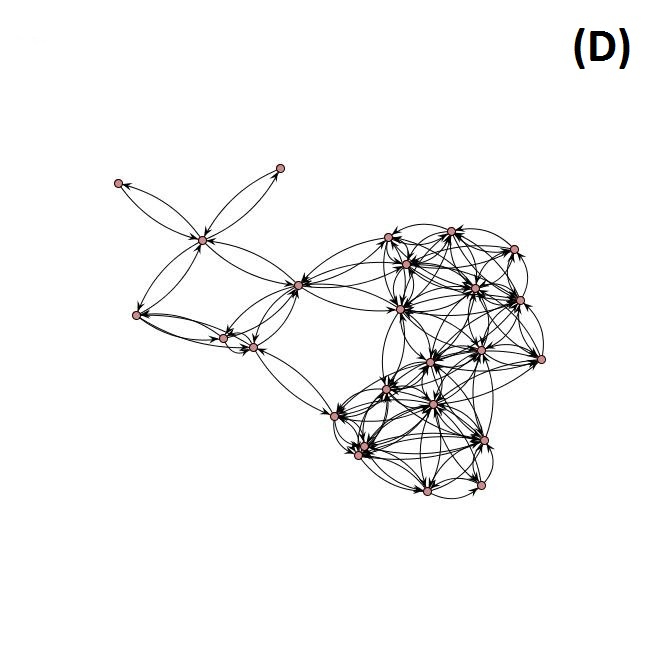
\includegraphics[width=0.3\linewidth]{../ExploratoryModelAnalysis/MDN/lcptest_MDN-D85_r0_sl50_j0}
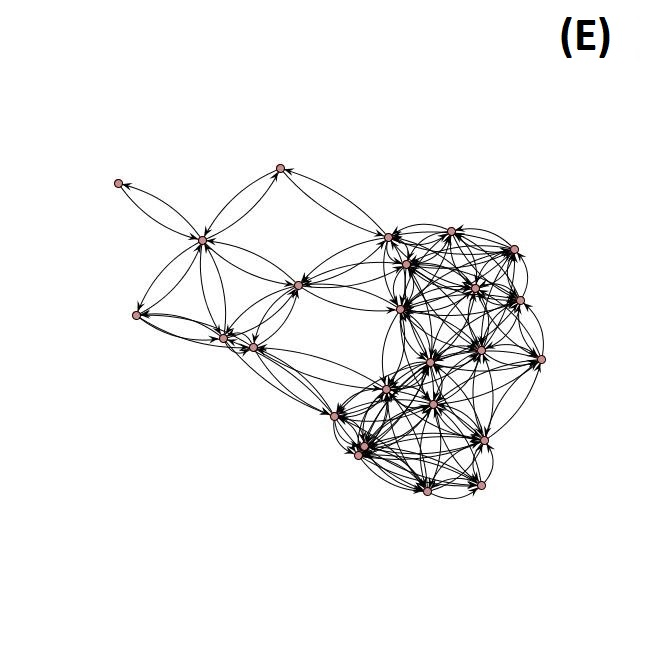
\includegraphics[width=0.3\linewidth]{../ExploratoryModelAnalysis/MDN/lcptest_MDN-D100_r0_sl50_j0}
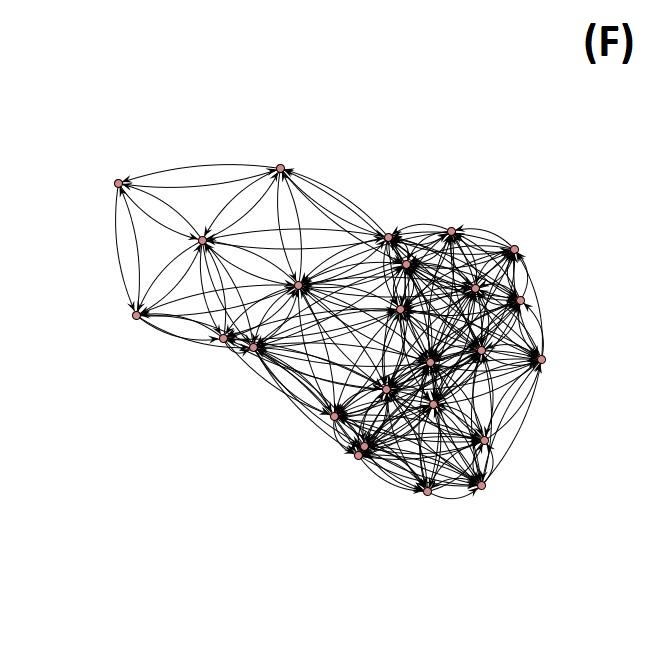
\includegraphics[width=0.3\linewidth]{../ExploratoryModelAnalysis/MDN/lcptest_MDN-D125_r0_sl50_j0}
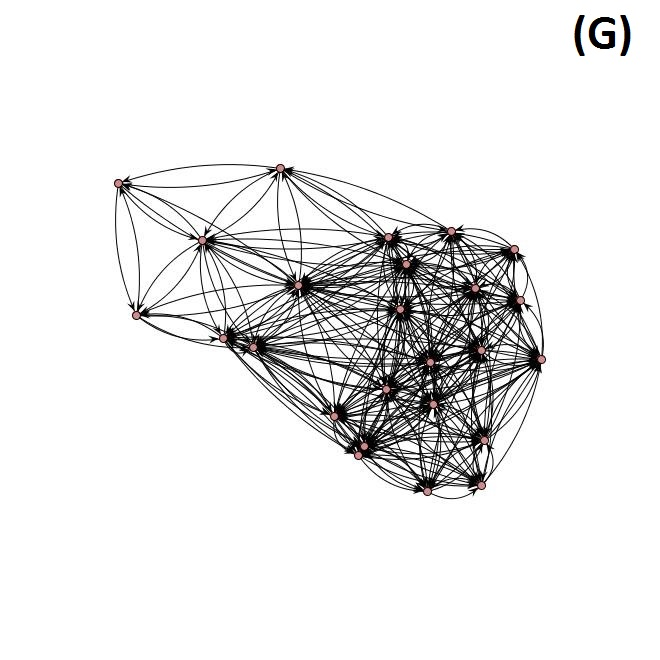
\includegraphics[width=0.3\linewidth]{../ExploratoryModelAnalysis/MDN/lcptest_MDN-D150_r0_sl50_j0}
\caption{A-G: MDN results for distance thresholds of 25km, 50km, 75km, 85km, 100km, 125km, and 150km.}
\label{fig:MDN}
\end{figure}

\begin{figure}
\centering
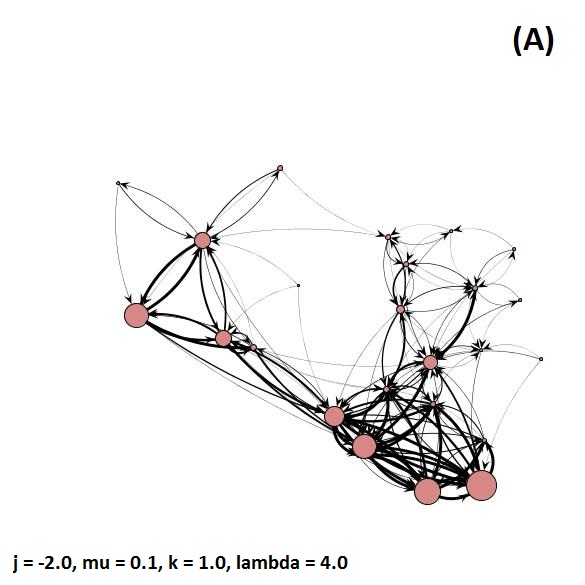
\includegraphics[width=0.3\linewidth]{../ExploratoryModelAnalysis/Ariadne/60/1lcptest_j-02_00-m00_100-k001_00-l004_00}
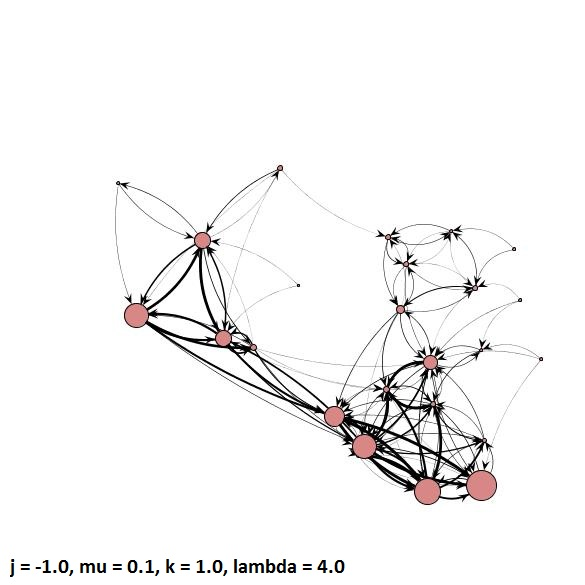
\includegraphics[width=0.3\linewidth]{../ExploratoryModelAnalysis/Ariadne/60/2lcptest_j-01_00-m00_100-k001_00-l004_00}
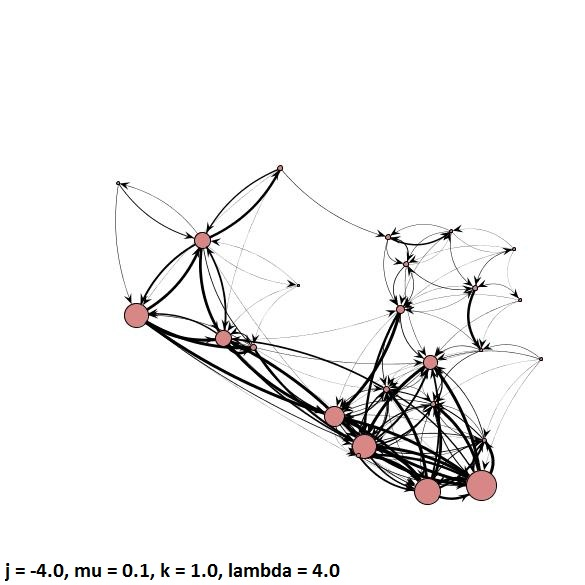
\includegraphics[width=0.3\linewidth]{../ExploratoryModelAnalysis/Ariadne/60/3lcptest_j-04_00-m00_100-k001_00-l004_00}
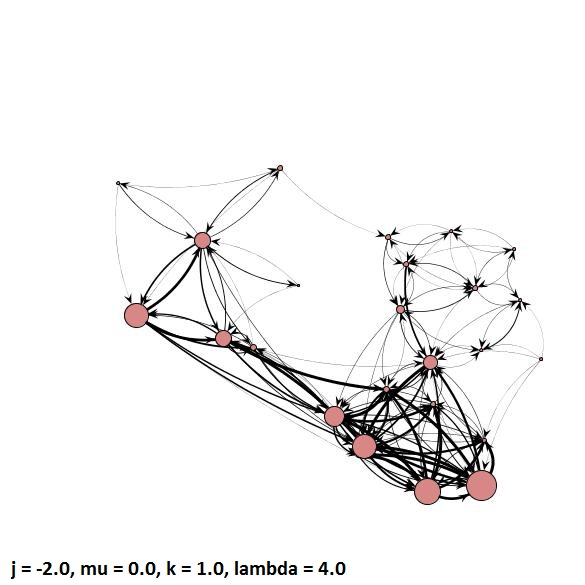
\includegraphics[width=0.3\linewidth]{../ExploratoryModelAnalysis/Ariadne/60/4lcptest_j-02_00-m000_00-k001_00-l004_00}
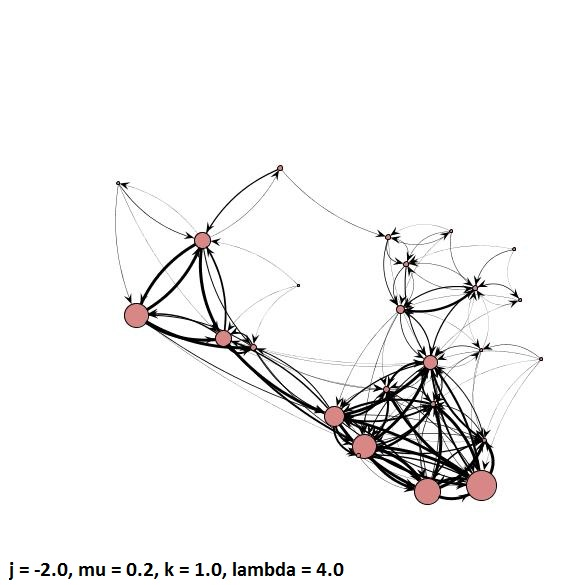
\includegraphics[width=0.3\linewidth]{../ExploratoryModelAnalysis/Ariadne/60/5lcptest_j-02_00-m00_200-k001_00-l004_00}
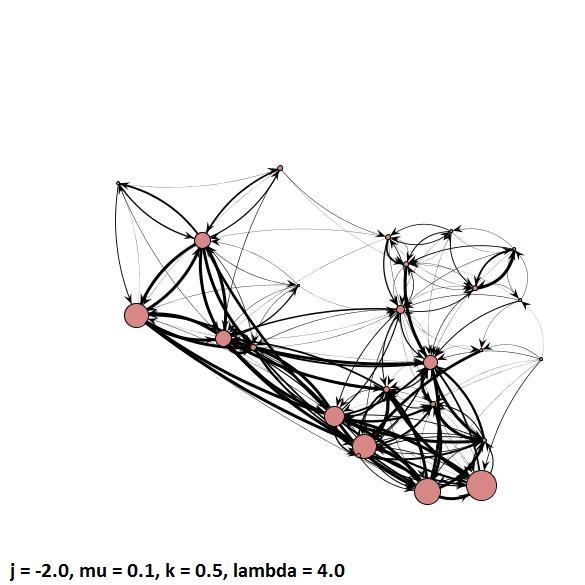
\includegraphics[width=0.3\linewidth]{../ExploratoryModelAnalysis/Ariadne/60/6lcptest_j-02_00-m00_100-k00_500-l004_00}
\includegraphics[width=0.3\linewidth]{../ExploratoryModelAnalysis/Ariadne/60/7lcptest_j-02_00-m00_100-k002_00-l004_00}
\includegraphics[width=0.3\linewidth]{../ExploratoryModelAnalysis/Ariadne/60/8lcptest_j-02_00-m00_100-k001_00-l002_00}
\includegraphics[width=0.3\linewidth]{../ExploratoryModelAnalysis/Ariadne/60/9lcptest_j-02_00-m00_100-k001_00-l008_00}
\caption{Parameterization of Ariadne (60km).}
\label{fig:60kmAll}
\end{figure}

\begin{figure}
\centering
\includegraphics[width=0.3\linewidth]{../ExploratoryModelAnalysis/Ariadne/100/1lcptest_j-02_00-m00_100-k001_00-l004_00}
\includegraphics[width=0.3\linewidth]{../ExploratoryModelAnalysis/Ariadne/100/2lcptest_j-01_00-m00_100-k001_00-l004_00}
\includegraphics[width=0.3\linewidth]{../ExploratoryModelAnalysis/Ariadne/100/3lcptest_j-04_00-m00_100-k001_00-l004_00}
\includegraphics[width=0.3\linewidth]{../ExploratoryModelAnalysis/Ariadne/100/4lcptest_j-02_00-m000_00-k001_00-l004_00}
\includegraphics[width=0.3\linewidth]{../ExploratoryModelAnalysis/Ariadne/100/5lcptest_j-02_00-m00_200-k001_00-l004_00}
\includegraphics[width=0.3\linewidth]{../ExploratoryModelAnalysis/Ariadne/100/6lcptest_j-02_00-m00_100-k00_500-l004_00}
\includegraphics[width=0.3\linewidth]{../ExploratoryModelAnalysis/Ariadne/100/7lcptest_j-02_00-m00_100-k002_00-l004_00}
\includegraphics[width=0.3\linewidth]{../ExploratoryModelAnalysis/Ariadne/100/8lcptest_j-02_00-m00_100-k001_00-l002_00}
\includegraphics[width=0.3\linewidth]{../ExploratoryModelAnalysis/Ariadne/100/9lcptest_j-02_00-m00_100-k001_00-l008_00}
\caption{Parameterization of Ariadne (100km).}
\label{fig:100kmAll}
\end{figure}

\begin{figure}
\centering
\tiny
\begin{tabular}{|c|c|c|c|c|c|c|c|}
\hline Run Number & Assortativity & Diameter & Average Degree & Transitivity & Beta & Gamma \\ 
\hline	5	&	-0.05140299	&	4.40000000	&	11.68000000	&	0.70671354	&	5.84000000	&	0.23360000	\\
\hline	10	&	-0.05091950	&	4.20000000	&	11.71200000	&	0.71293931	&	5.85600000	&	0.23424000	\\
\hline	15	&	-0.05081230	&	4.20000000	&	11.64266667	&	0.70496897	&	5.82133333	&	0.23285333	\\
\hline	20	&	-0.05107444	&	4.20000000	&	11.63600000	&	0.70794023	&	5.81800000	&	0.23272000	\\
\hline	25	&	-0.05119454	&	4.16000000	&	11.62880000	&	0.70893446	&	5.81440000	&	0.23257600	\\ 
\hline 
\end{tabular}
\caption{Network-level metric results for 25 runs (Ariadne - Before - 60km)}
\label{fig:ConvergeAriadneB60} 
\end{figure}

\begin{figure}
\centering
\tiny
\begin{tabular}{|c|c|c|c|c|c|c|c|}
\hline Run Number & Assortativity & Diameter & Average Degree & Transitivity & Beta & Gamma \\ 
\hline	5	&	-0.05526671	&	3.00000000	&	12.14400000	&	0.73106504	&	6.07200000	&	0.24288000	\\
\hline	10	&	-0.05538473	&	3.00000000	&	11.84800000	&	0.69957622	&	5.92400000	&	0.23696000	\\
\hline	15	&	-0.05541665	&	3.13333333	&	11.96800000	&	0.70008067	&	5.98400000	&	0.23936000	\\
\hline	20	&	-0.05569742	&	3.10000000	&	11.63600000	&	0.69305360	&	5.81800000	&	0.23272000	\\
\hline	25	&	-0.05581519	&	3.12000000	&	11.65760000	&	0.69901818	&	5.82880000	&	0.23315200	\\
\hline 
\end{tabular}
\caption{Network-level metric results for 25 runs (Ariadne - Before - 100km)}
\label{fig:ConvergeAriadneB100} 
\end{figure}

\begin{figure}
\centering
\tiny
\begin{tabular}{|c|c|c|c|c|c|c|c|}
\hline Run Number & Assortativity & Diameter & Average Degree & Transitivity & Beta & Gamma \\ 
\hline	5	&	-0.05294613	&	4.60000000	&	11.42400000	&	0.71058266	&	5.95000000	&	0.24791667	\\
\hline	10	&	-0.05346564	&	4.50000000	&	11.18400000	&	0.71911467	&	5.82500000	&	0.24270833	\\
\hline	15	&	-0.05322030	&	4.33333333	&	11.24266667	&	0.72488791	&	5.85555556	&	0.24398148	\\
\hline	20	&	-0.05322119	&	4.25000000	&	11.37600000	&	0.72831435	&	5.92500000	&	0.24687500	\\
\hline	25	&	-0.05325428	&	4.24000000	&	11.31520000	&	0.72501267	&	5.89333333	&	0.24555556	\\
\hline 
\end{tabular}
\caption{Network-level metric results for 25 runs (Ariadne - After - 60km)}
\label{fig:ConvergeAriadneA60} 
\end{figure}

\begin{figure}
\centering
\tiny
\begin{tabular}{|c|c|c|c|c|c|c|c|}
\hline Run Number & Assortativity & Diameter & Average Degree & Transitivity & Beta & Gamma \\ 
\hline	5	&	-0.05840201	&	3.20000000	&	10.46400000	&	0.66037357	&	5.45000000	&	0.22708333	\\
\hline	10	&	-0.05642575	&	3.10000000	&	10.87200000	&	0.67265716	&	5.66250000	&	0.23593750	\\
\hline	15	&	-0.05726372	&	3.06666667	&	11.03466667	&	0.69067383	&	5.74722222	&	0.23946759	\\
\hline	20	&	-0.05687748	&	3.10000000	&	11.01200000	&	0.68319655	&	5.73541667	&	0.23897569	\\
\hline	25	&	-0.05695306	&	3.08000000	&	10.91840000	&	0.67954338	&	5.68666667	&	0.23694444	\\
\hline 
\end{tabular}
\caption{Network-level metric results for 25 runs (Ariadne - After - 100km)}
\label{fig:ConvergeAriadneA100} 
\end{figure}


\begin{figure}
\centering
\includegraphics[width=0.35\linewidth]{../BeforeViz/agentTest1}
\includegraphics[width=0.35\linewidth]{../BeforeViz/agentTest2}
\includegraphics[width=0.35\linewidth]{../BeforeViz/agentTest3}
\includegraphics[width=0.35\linewidth]{../BeforeViz/agentTest4}
\includegraphics[width=0.35\linewidth]{../BeforeViz/agentTest5}
\caption{Five sample model runs for the agent model.}
\label{fig:agentFluctuations}
\end{figure}


\begin{figure}
\centering
\tiny
\begin{tabular}{|c|c|c|c|c|c|c|c|}
\hline Run Number & Assortativity & Diameter & Average Degree & Transitivity & Beta & Gamma \\ 
\hline	5	&	-0.04980000	&	5.00000000	&	8.37000000	&	0.43800000	&	4.18000000	&	0.16700000	\\
\hline	10	&	-0.04030000	&	5.00000000	&	8.36000000	&	0.44100000	&	4.18000000	&	0.16700000	\\
\hline	15	&	-0.03890000	&	5.00000000	&	8.42000000	&	0.43600000	&	4.21000000	&	0.16800000	\\
\hline	20	&	-0.04120000	&	5.00000000	&	8.39000000	&	0.43500000	&	4.20000000	&	0.16800000	\\
\hline	25	&	-0.03900133	&	5.00000000	&	8.31360000	&	0.43295384	&	4.15680000	&	0.16627200	\\
\hline 
\end{tabular}
\caption{Network-level metric results for 25 runs (Agent Model - Before)}
\label{fig:ConvergeAgentB} 
\end{figure}

\begin{figure}
\centering
\tiny
\begin{tabular}{|c|c|c|c|c|c|c|c|}
\hline Run Number & Assortativity & Diameter & Average Degree & Transitivity & Beta & Gamma \\ 
\hline	5 &	-0.02416639	&	5.00000000	&	7.93600000	&	0.43904952 &	4.13333333	&	0.17222222	\\
\hline	10 & -0.02245842	&	5.00000000	&	7.92000000	&	0.43448981	&	4.12500000	&	0.17187500	\\
\hline	15 & -0.02198818	&	5.00000000	&	7.94666667	&	0.43704930	&	4.13888889	&	0.17245370	\\
\hline	20 & -0.02568726	&	5.00000000	&	7.96000000	&	0.44110698	&	4.14583333	&	0.17274306	\\
\hline	25 & -0.02370421	&	5.00000000	&	7.97440000	&	0.44168669	&	4.15333333	&	0.17305556	\\
\hline 
\end{tabular}
\caption{Network-level metric results for 25 runs (Agent Model - After)}
\label{fig:ConvergeAgentA} 
\end{figure}


\end{appendices}

\end{document}}